%% ----------------------------------------------------------------
%% Thesis.tex -- MAIN FILE (the one that you compile with LaTeX)
%% ---------------------------------------------------------------- 

% Set up the document
\documentclass[a4paper, 11pt, oneside]{uet_thesis}  % Use the "Thesis" style, based on the ECS Thesis style by Steve Gunn
\graphicspath{{Figures/}}  % Location of the graphics files (set up for graphics to be in PDF format)

% Include any extra LaTeX packages required
\usepackage[square, numbers, comma, sort&compress]{natbib}  % Use the "Natbib" style for the references in the Bibliography

\usepackage{verbatim}  % Needed for the "comment" environment to make LaTeX comments

\usepackage{vector}  % Allows "\bvec{}" and "\buvec{}" for "blackboard" style bold vectors in maths

\usepackage{url}
\usepackage{natbib}

\usepackage{listings}
\usepackage{color}

\definecolor{dkgreen}{rgb}{0,0.6,0}
\definecolor{gray}{rgb}{0.5,0.5,0.5}
\definecolor{mauve}{rgb}{0.58,0,0.82}
\definecolor{light_gray}{rgb}{0.95,0.95,0.95}

\lstset{
	backgroundcolor=\color{light_gray},
	frame=TB,
	captionpos=b,
	escapeinside={(*@}{@*)},
	language=C,
	aboveskip=3mm,
	belowskip=3mm,
	showstringspaces=false,
	columns=flexible,
	basicstyle={\small\ttfamily},
	numbers=none,
	numberstyle=\tiny\color{gray},
	keywordstyle=\color{blue},
	commentstyle=\color{dkgreen},
	stringstyle=\color{mauve},
	breaklines=true,
	breakatwhitespace=true,
	tabsize=3
}


\hypersetup{urlcolor=blue, colorlinks=true}  % Colours hyperlinks in blue, but this can be distracting if there are many links.

% remove the unnecessary spacing before and after the headings/subheadings
\usepackage[compact]{titlesec}
\titlespacing{\section}{0pt}{*0}{*0}
\titlespacing{\subsection}{0pt}{*0}{*0}
\titlespacing{\subsubsection}{0pt}{*0}{*0}

\setlength{\parskip}{6pt}
%\setlength{\parsep}{0pt}
%\setlength{\headsep}{0pt}
%\setlength{\topskip}{0pt}

%% ----------------------------------------------------------------
\begin{document}
\frontmatter	  % Begin Roman style (i, ii, iii, iv...) page numbering

% Set up the Title Page
\title  {Project Report \linebreak
Cascaded H-Bridge Inverter with 9 Levels in Voltage Waveform
}
\session {2017 -- 2021}
\advisor {Sir Aneeq Aslam}
\authors {
Usman IlamDin ~~~~~~~~~~~~~~ 2017-EE-119\\
Arslan Shafique ~~~~~~~~~~~~~~~2017-EE-118\\
Khawaja ~~~~~~~~~~~2017-EE-135\\
Hamza Naseer ~~~~~~~~~~~~~~ 2017-EE-149 }

\addresses  {\deptname \\ \univname}  % Do not change this here, instead these must be set in the "Thesis.cls" file, please look through it instead
\date       {\today}
\subject    {}
\keywords   {}

\maketitle
%% ----------------------------------------------------------------

\setstretch{1.3}  % It is better to have smaller font and larger line spacing than the other way round

% Define the page headers using the FancyHdr package and set up for one-sided printing
\fancyhead{}  % Clears all page headers and footers
\rhead{\thepage}  % Sets the right side header to show the page number
\lhead{}  % Clears the left side page header

\pagestyle{fancy}  % Finally, use the "fancy" page style to implement the FancyHdr headers


%% Select only one of the certification pages  
%\CertificationMSc{}
%\CertificationBSc{}
%\clearpage  % Certification ended, now start a new page


%% ----------------------------------------------------------------
% Declaration Page required for the Thesis, your institution may give you a different text to place here
\Declaration{
\addtocontents{toc}{\vspace{1em}}  % Add a gap in the Contents, for aesthetics

We declare that the work contained in this thesis/report is my own, except where explicitly stated otherwise. In addition this work has not been submitted to obtain another degree or professional qualification.

\bigskip

Signed:~~ \rule[0em]{10em}{1.0pt} \\ % This prints a line for the signature 
Signed:~~ \rule[0em]{10em}{1.0pt} \\ % This prints a line for the signature \\
Signed:~~ \rule[0em]{10em}{1.0pt} \\ % This prints a line for the signature \\
Signed:~~ \rule[0em]{10em}{1.0pt} \\ % This prints a line for the signature 
Date:~~~~ \rule[0em]{10em}{1.0pt}  % This prints a line to write the date
}
\clearpage     % Declaration ended, now start a new page

%% ----------------------------------------------------------------

%\setstretch{1.3}  % Reset the line-spacing to 1.3 for body text (if it has changed)

% The Acknowledgements page, for thanking everyone
%\acknowledgements{
%\addtocontents{toc}{\vspace{1em}}  % Add a gap in the Contents, for aesthetics

%The acknowledgements and the people to thank go here, don't forget to include your project advisor\ldots

%}
%\clearpage  % End of the Acknowledgements

%% ----------------------------------------------------------------
% End of the pre-able, contents and lists of things
% Begin the Dedication page
%\setstretch{1.3}  % Return the line spacing back to 1.3
%\pagestyle{empty}  % Page style needs to be empty for this page
%\dedicatory{For/Dedicated to/To my\ldots}


%% ----------------------------------------------------------------
%\pagestyle{fancy}  %The page style headers have been "empty" all this time, now use the "fancy" headers as defined before to bring them back

%% ----------------------------------------------------------------
\lhead{\emph{Contents}}  % Set the left side page header to "Contents"
\tableofcontents 
 % Write out the Table of Contents

%% ----------------------------------------------------------------
\lhead{\emph{List of Figures}}  % Set the left side page header to "List if Figures"
\listoffigures  % Write out the List of Figures

%% ----------------------------------------------------------------
%\lhead{\emph{List of Tables}}  % Set the left side page header to "List of Tables"
%\listoftables  % Write out the List of Tables

%% ----------------------------------------------------------------
\setstretch{1.5}  % Set the line spacing to 1.5, this makes the following tables easier to read
\clearpage  % Start a new page
%\lhead{\emph{Abbreviations}}  % Set the left side page header to "Abbreviations"
%\listofsymbols{ll}  % Include a list of Abbreviations (a table of two columns)
{
% \textbf{Acronym} & \textbf{W}hat (it) \textbf{S}tands \textbf{F}or \\
%\textbf{LAH} & \textbf{L}ist \textbf{A}bbreviations \textbf{H}ere \\
}

%% ----------------------------------------------------------------
% The Abstract Page
\addtotoc{Abstract}  % Add the "Abstract" page entry to the Contents
\abstract{
\addtocontents{toc}{\vspace{1em}}  % Add a gap in the Contents, for aesthetics

Cascaded H-Bridge Multilevel Inverters 
can generate high quality voltage waveforms close to sinusoidal.CHB Multilevel inverter that is constituted using dual H-bridge cells
with MOSFETs on each phase legs. The output waveform is increased up to 9-level by using 2 separate DC sources defined at Vdc:3Vdc ratio to obtain an asymmetrical output. The cascaded multilevel inverter is switched by the proposed SPWM
modulator. The harmonic analysis of proposed inverter has been
performed under several working conditions such as various
switching frequencies and modulation indexes. The detailed
comparisons are performed to determine the best working
conditions of voltage source inverters (VSI) and presented in this
report.\ldots

%}
\clearpage  % Abstract ended, start a new page

%% ----------------------------------------------------------------
\mainmatter	  % Begin normal, numeric (1,2,3...) page numbering
\pagestyle{fancy}  % Return the page headers back to the "fancy" style
\onehalfspacing
% Include the chapters of the thesis, as separate files
% Just uncomment the lines as you write the chapters

%chapter 1

\chapter{Introduction} % Write in your own chapter title
\label{Chapter0}
\lhead{Chapter 0. \emph{Introduction}} % Write in your own chapter title to set the page header

\section{Motivation}
The main objective or motivation of this report is to increase the knowledge about the concepts of Power Electronics. To practically apply all the concepts and prove them. This project is simulations based and is being done on Simulink ,Matlab. In this we have Simulated the three type of circuits which covers most of the power electronics course and have matched the simulated results with the theoretical ones. The building blocks of the project are rectifier ,inverter and LCL filter. The industrial application of this in the ups in which AC is first converted into DC which is used for charging the batteries and the output of batteries which is DC voltage is then converted into AC through inverters. 

\section{Problem Statment}
The problem given in the statement is to first input the three phase AC source whose magnitude is to be 400V. The three phases are displaced by 120 degrees as in case of practical ones. Then the input is to be passed through rectifier which converts it into DC. The Rectifier we have used in this case in controlled rectifier whose firing angle  can be adjusted such that we can vary the the output voltage. The gate pulses are used for controlling the firing angle .The gate pulses are such that no thristors of same leg will be on at the time instant  .The output voltage is 400Vdc. This DC voltage is then fed into the inverter circuit. The inverter being used is three phase sine-pwm. The inverter converts the dc voltage into three phase AC. The three phase AC is such that it contains the steps. The three steps are then converted into the sine waveform using the LCL filter. The filter is designed such that the output voltage is pure sine waveform.    
 % Introduction 

% Chapter 1

\chapter{Flow Chart and Block Diagram} % Write in your own chapter title
\label{Chapter2}
\lhead{Chapter 2. \emph{Flow Chart and Block Diagram}} % Write in your own chapter title to set the page header
\section{Flowchart}

\begin{figure}[htbp]
	\centering
		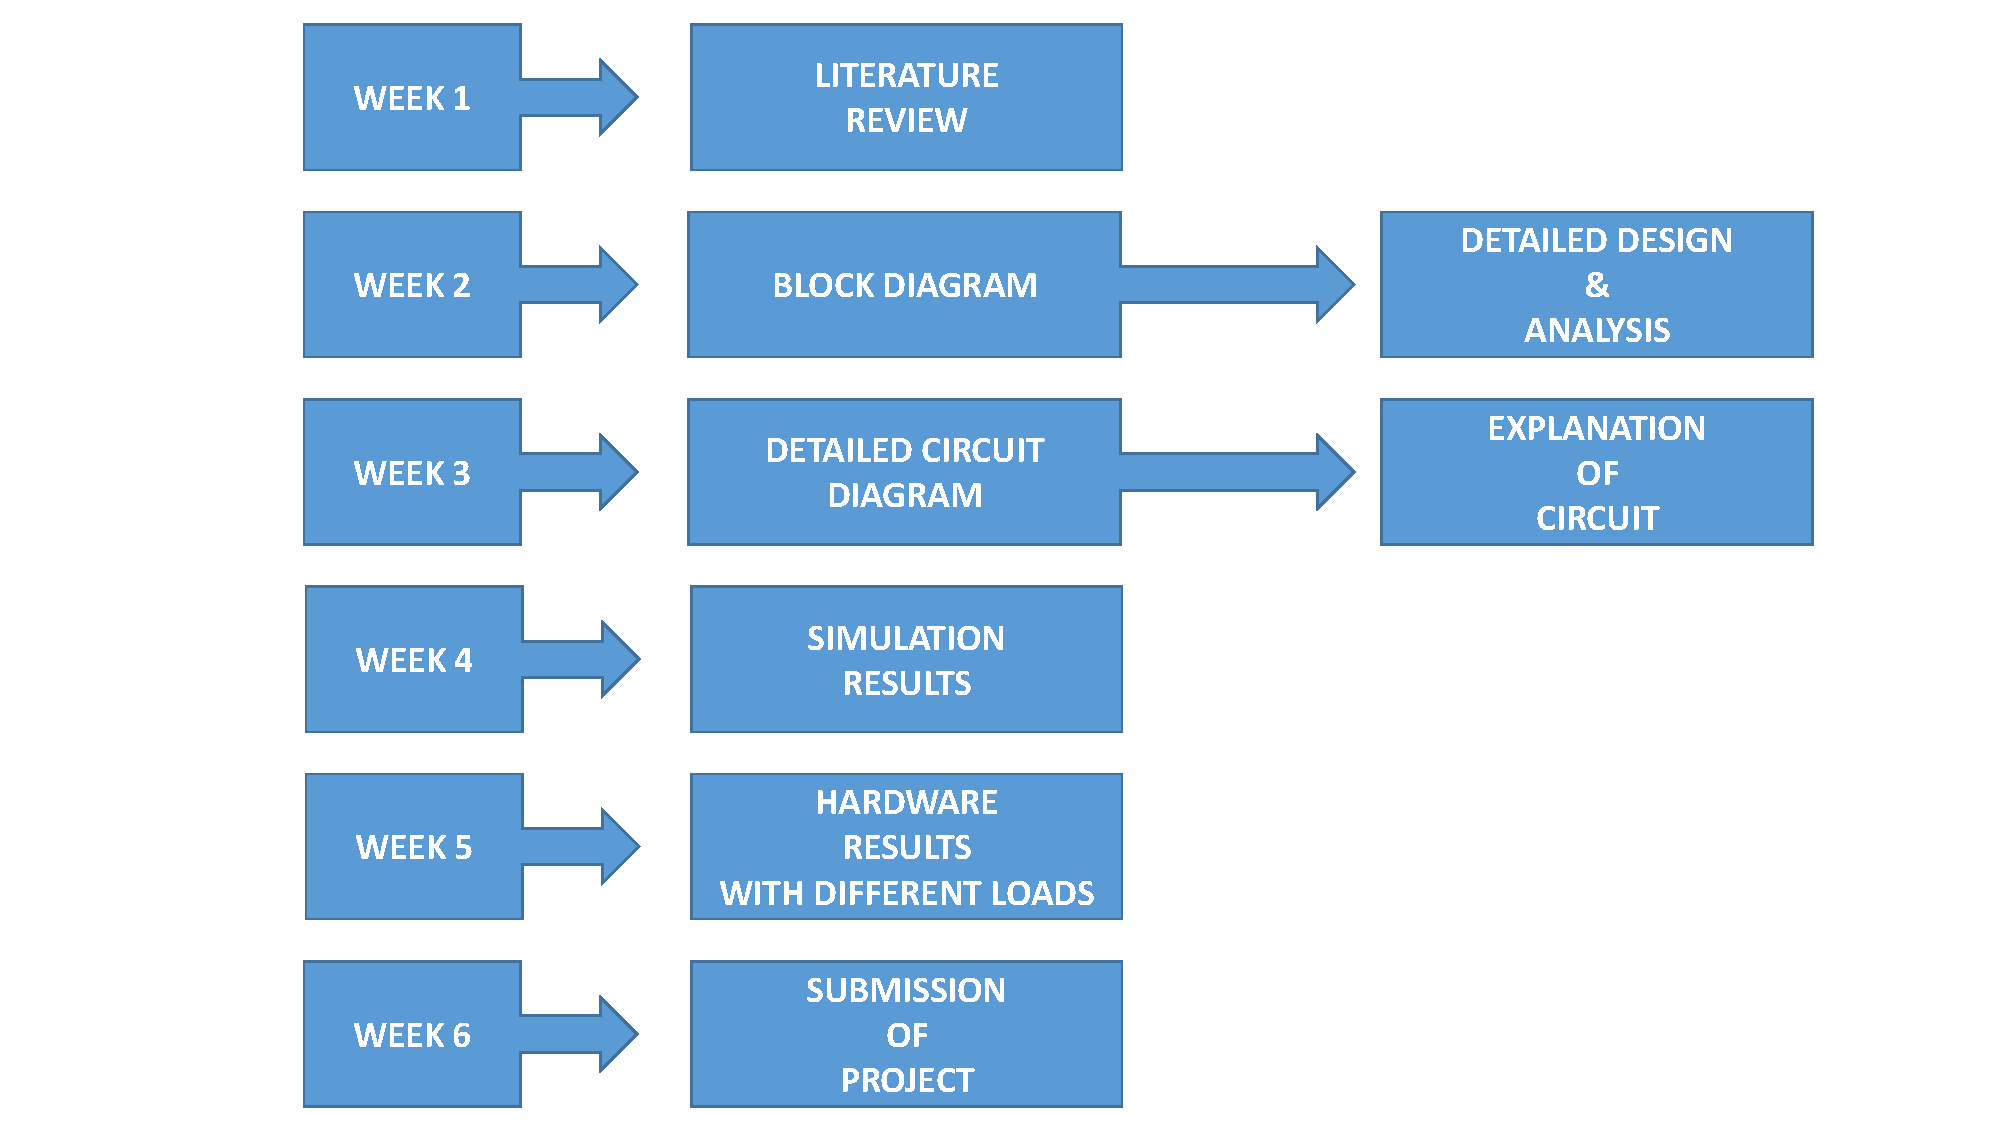
\includegraphics[width = 7in]{./Figures/Presentation1.pdf}
		\rule{35em}{5pt}
	\caption{Flowchart of Project Progress}
	\label{fig:1}
\end{figure}
\newpage
\section{Block Diagram}
\begin{figure}[htbp]
	\centering
		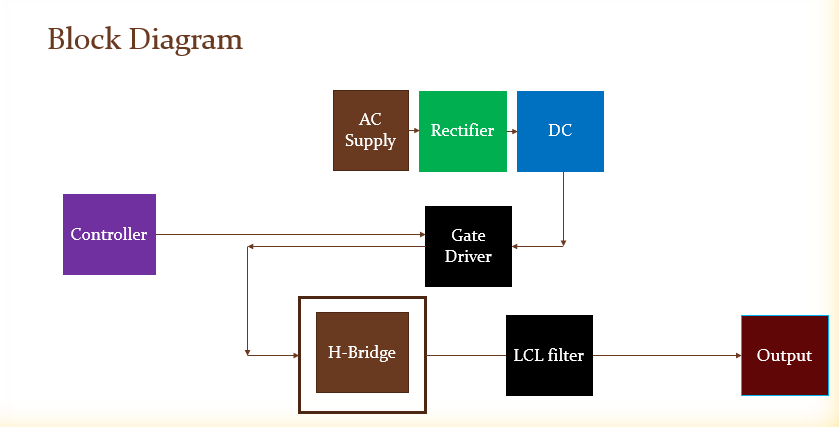
\includegraphics[width = 5in]{./Figures/block}
		\rule{35em}{5pt}
	\caption{Block Diagram of Project Progress}
	\label{fig:2}
\end{figure} % What to Write 

% Chapter 1

\chapter{Software Implementation} % Write in your own chapter title
\label{Chapter2}
\lhead{Chapter 2. \emph{Software Implementation}} % Write in your own chapter title to set the page header
\section{Block Diagram}
\begin{tikzpicture}[]
	\node  (in1) [above=1cm,io, label={[yshift=-0.5cm]left:Input-\\ three-\\phase}]{};
	\node  (in2) [below=1cm of in1, io]{};
	\node (out1) [right= 13cm of in1]{};
	\node (out2) [right= 13cm of in2]{};
	\draw (in1)--node[pos=0.8,above=2pt]{$I_{out}$}(out1);
	\draw (in2)--(out2);
	\path (in1)--node[pos=0.5](a){}(in2)
	node[block,right=1cm of a](t){Rect-\\tifier}
	node[block,right=1cm of t](r){Filter}
	node[block,right=1cm of r](f){Inverter} 
	node[block,right=1cm of f](re){LCLfilter}
	node[block,right=1cm of re](l){Load}
	;
	\draw[->] (11,1.2)--+(0.5,0);
	\node[above right=0.2cm and 1cm] at (re){$+$};
	\node[right=1cm] at (re){$V_{out}$};
	\node[below right=0.2cm and 1cm] at (re){$-$};
	\pic at (2.5,2) [scale=0.2]{reti};
	\pic at (5.5,-2) [scale=0.2]{filted};
	\pic at (8,2) [scale=0.2]{mysine};
\end{tikzpicture}

\section{Rectifier}
Below is the Matlab Simulink Diagram of Controlled Rectifier
\begin{figure}[htbp]
	\centering
	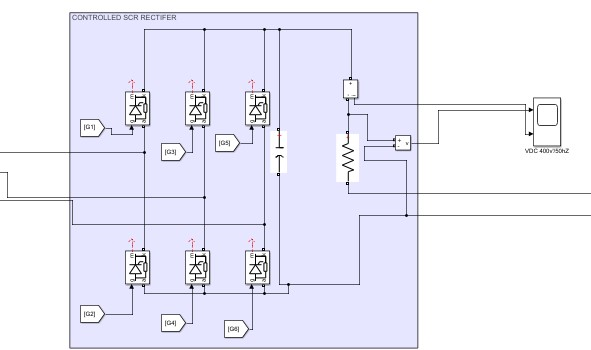
\includegraphics[width = 6in]{./Figures/rectifier1.jpg}
	\rule{35em}{1pt}
	\caption{Controlled Rectifier Block}
\end{figure}
The Controlled gate pulse Simulink Diagram
\begin{figure}[htbp]
	\centering
	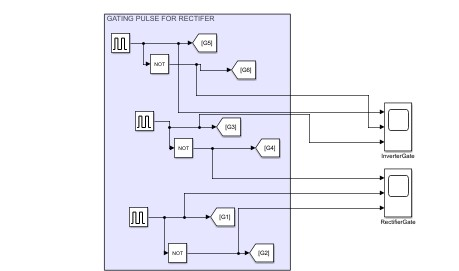
\includegraphics[width = 6in]{./Figures/rectifier2.jpg}
	\rule{35em}{1pt}
	\caption{Controlled Pulse Block}
\end{figure}
\newpage
\section{Inverter}
\subsection{SPWM Inverter}
\begin{figure}[htbp]
	\centering
	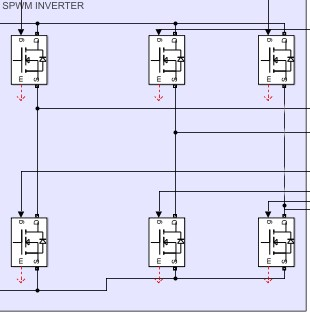
\includegraphics[width = 6in]{./Figures/Inverter.jpg}
	\rule{35em}{1pt}
	\caption{Inverter Block}
\end{figure}

\begin{figure}[htbp]
	\centering
	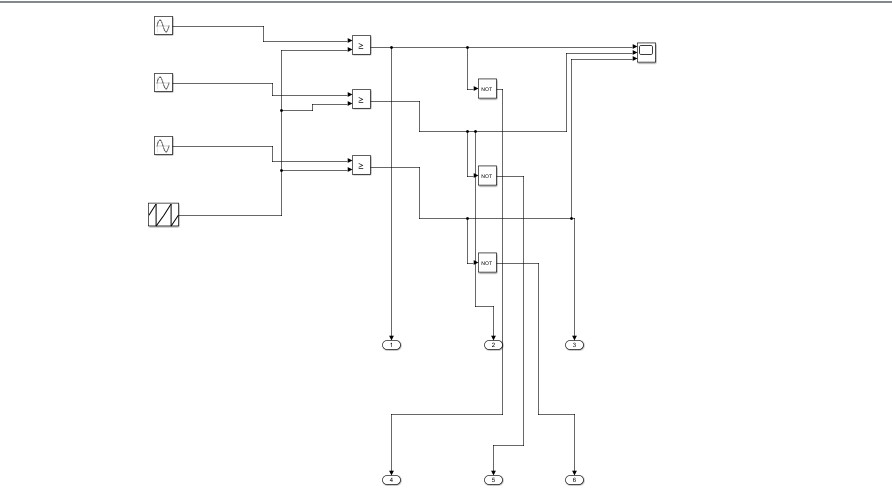
\includegraphics[width = 6in]{./Figures/Inverter1.jpg}
	\rule{35em}{1pt}
	\caption{Controlled Pulse Block}
\end{figure}
\newpage
\subsection{180 consuction Inverter}
\begin{figure}[htbp]
	\centering
	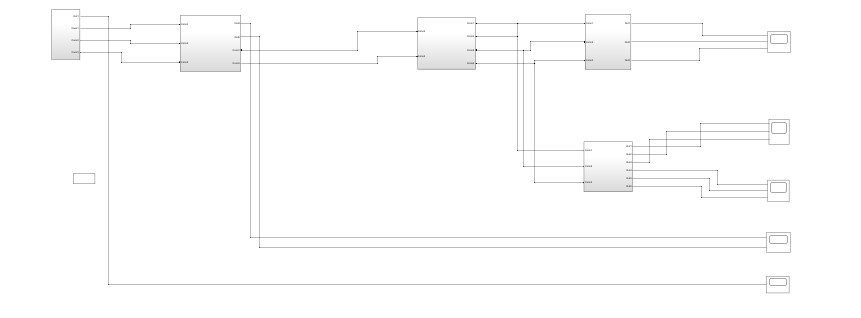
\includegraphics[width = 6in]{./Figures/180inverter.jpg}
	\rule{35em}{1pt}
	\caption{Simulink Diagram}
\end{figure}
\begin{figure}[htbp]
	\centering
	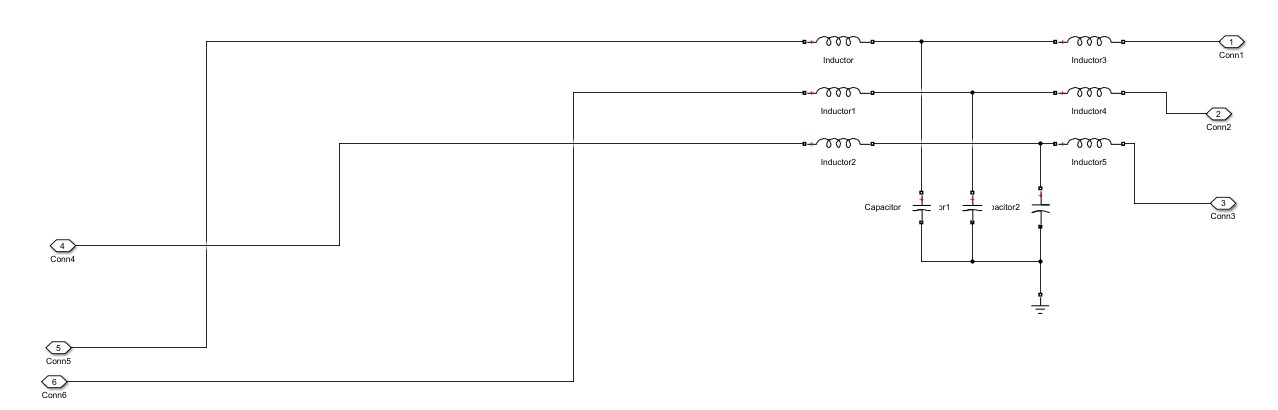
\includegraphics[width = 6in]{./Figures/LCL.jpg}
	\rule{35em}{1pt}
	\caption{LCL filter}
\end{figure} % Experimental Setup
 
% Chapter 1

\chapter{Detailed Circuit Design} % Write in your own chapter title
\label{Chapter4}
\lhead{Chapter 4. \emph{Detailed Circuit Design}} % Write in your own chapter title to set the page header
The complete circuit diagram of the circuit is shown\ref{fig:1}. 
\begin{figure}[htbp]
	
		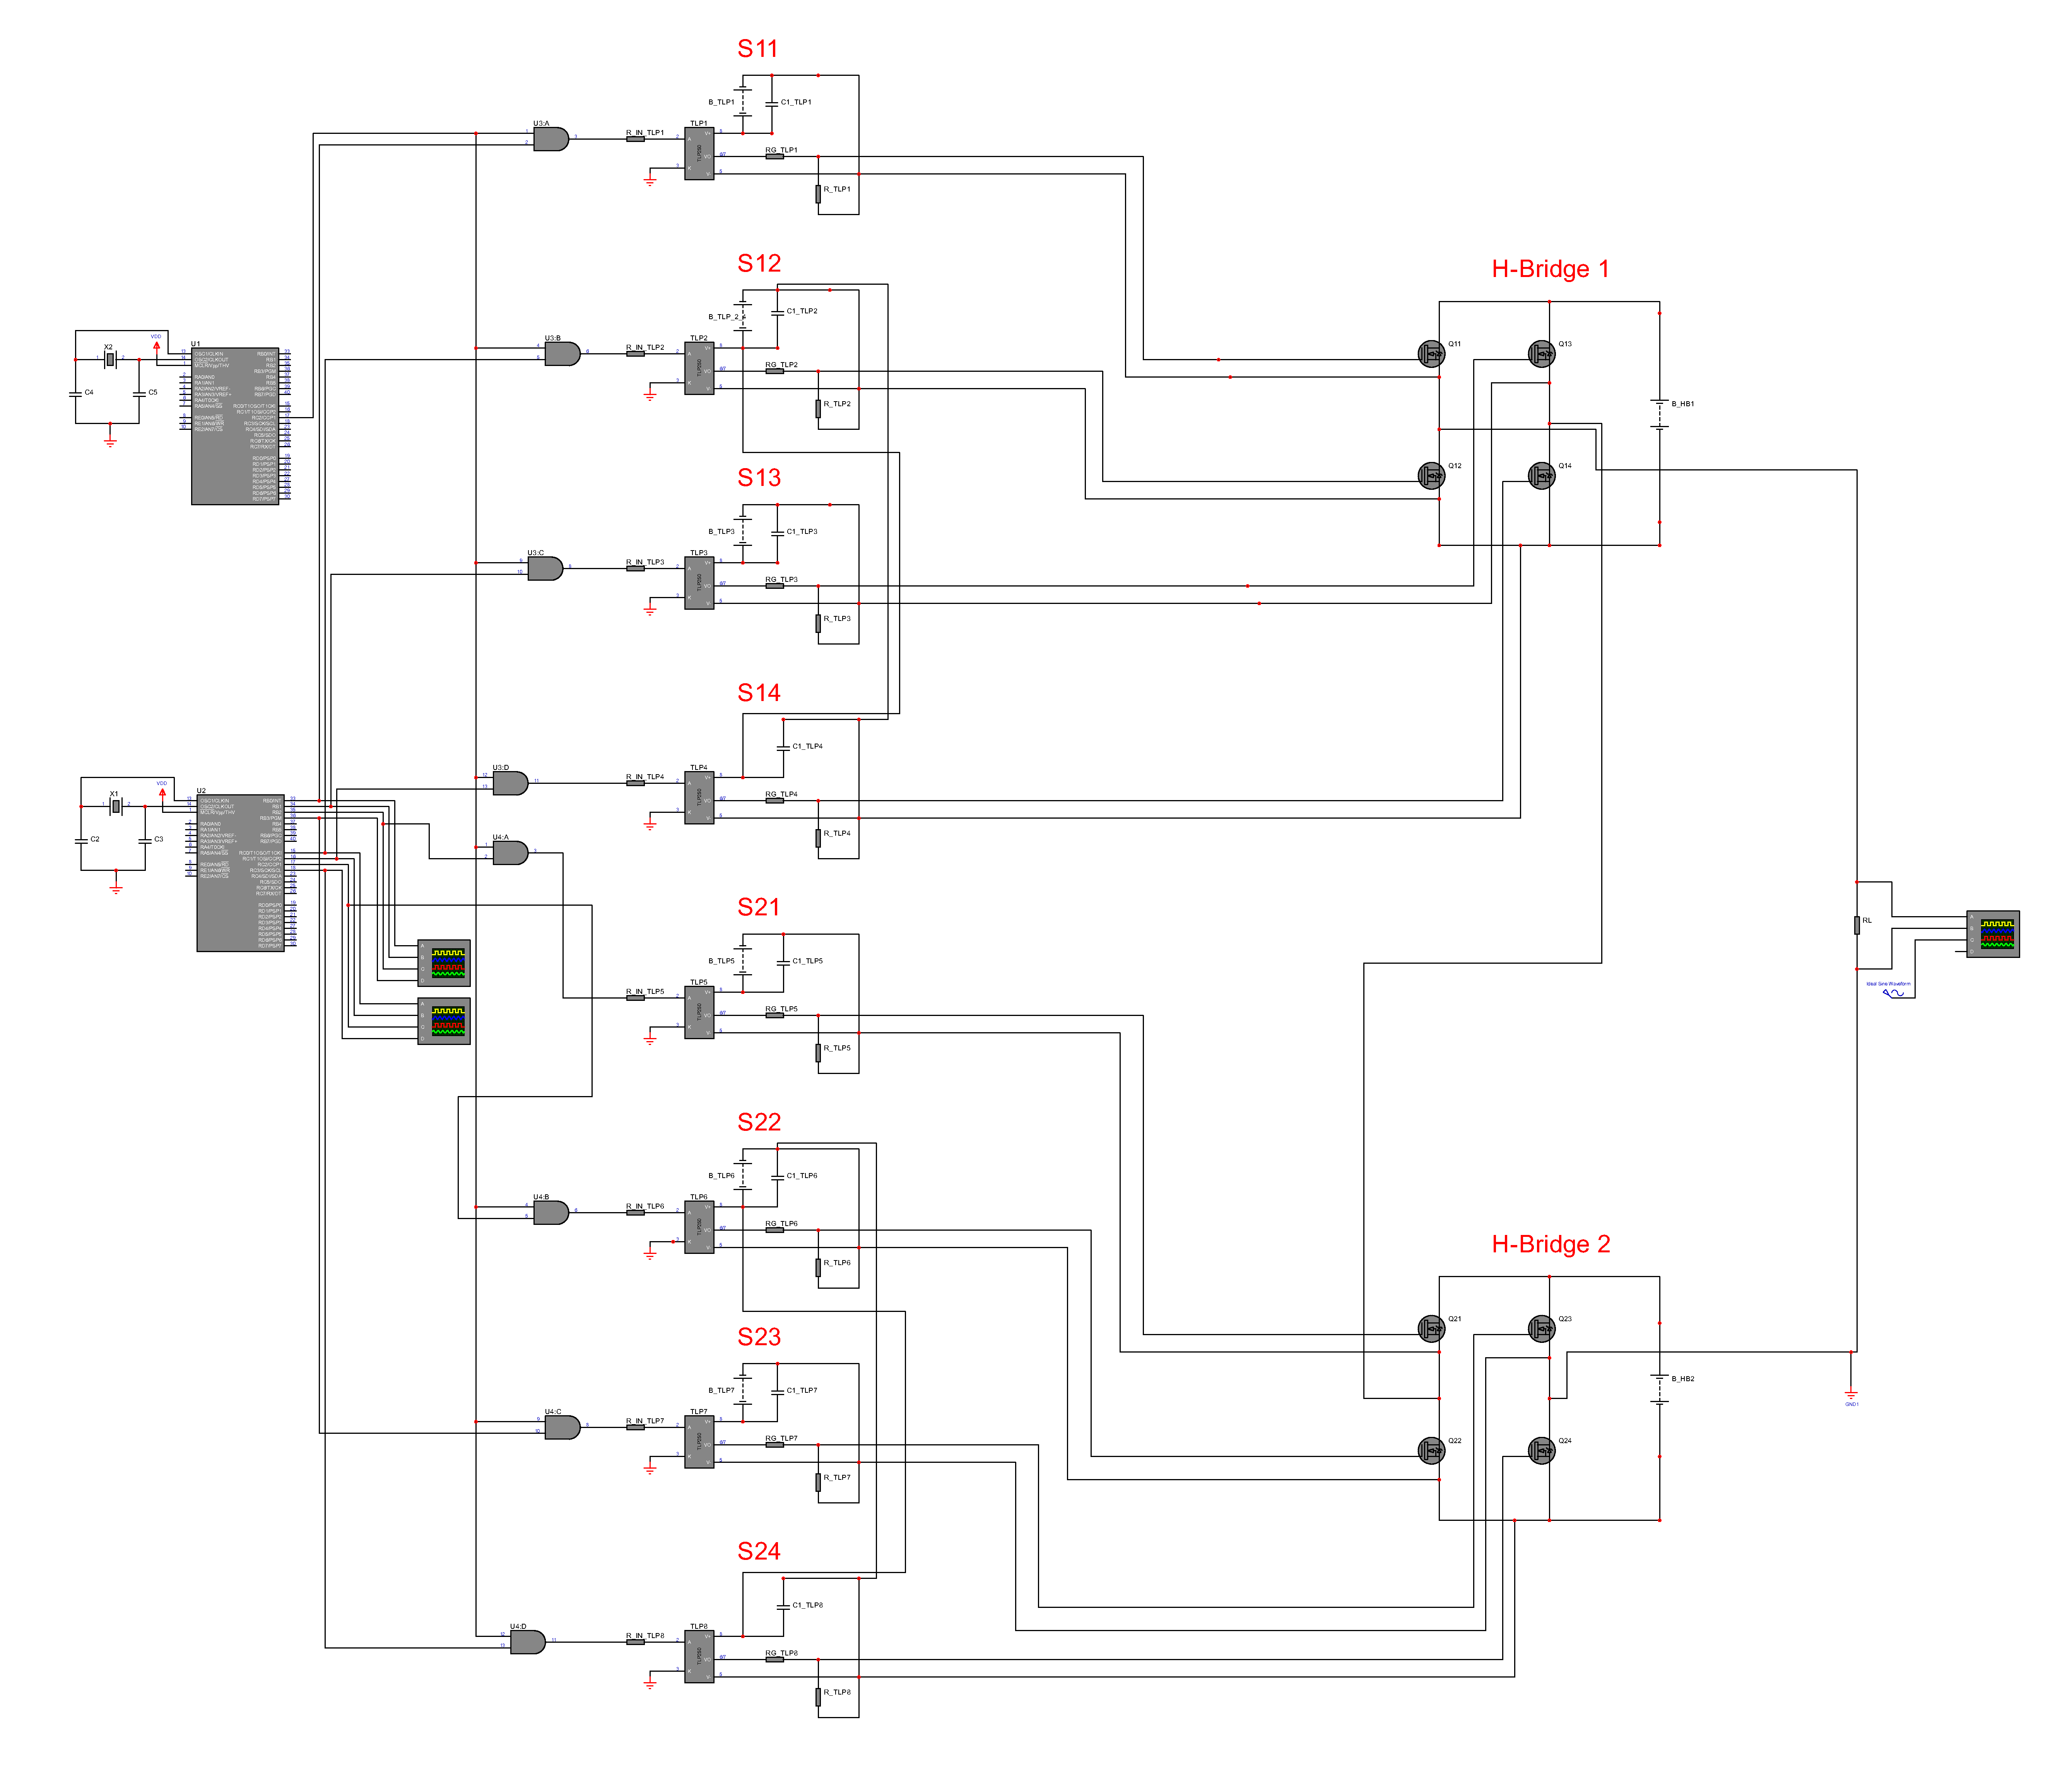
\includegraphics[width = 6in]{./Figures/Photos/circuit.pdf}
		\rule{35em}{2pt}
	\caption{Circuit for 9 Levels Voltage wave-forms}
	\label{fig:1}
\end{figure}
\newpage
The circuit\ref{fig:1} is divided into 4 main portions as:
\begin{itemize}
\item DC Supplies.
\item STM32F4x Micro-controller to apply switching.
\item Gate Triggering Circuit using Opto-coupler TLP250.
\item 2 Cascaded H-Bride Inverter.
\end{itemize}
\section{DC Supplies}
In this circuit total 8 DC supplies are used to power the circuit,6(Isolated) out of them have 15 Volts output to power the TLP 250 present in Gate triggering circuit.and the other two having outputs ratio of 1:3 vollts are used to get 9 levels output voltage waveform.Gate Drivers for ground connected Mosfets have given same supply.
\begin{figure}[htbp]
	\centering
		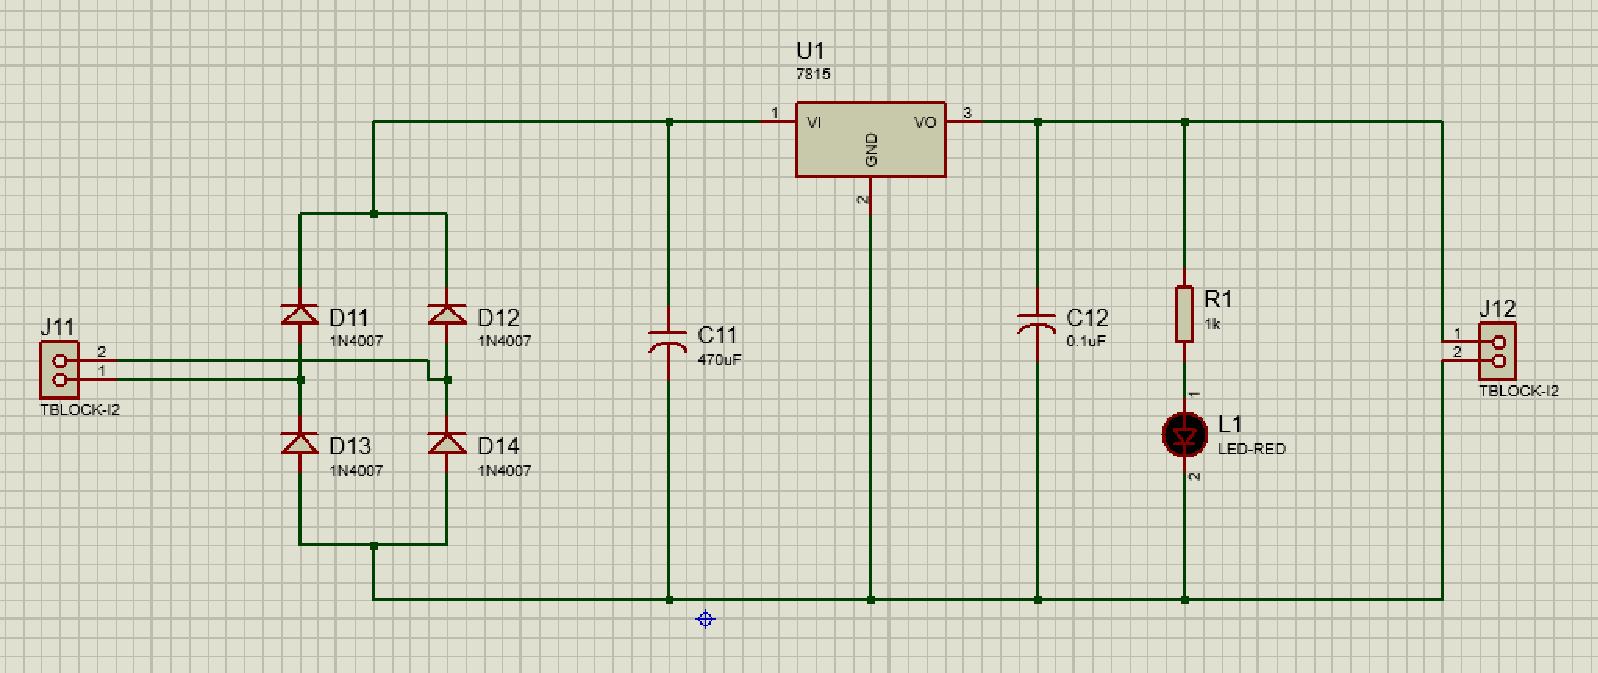
\includegraphics[width = 5in]{./Figures/ss.pdf}
		\rule{35em}{5pt}
	\caption{Circuit for Constant DC supply}
	\label{fig:2}
\end{figure}
\section{STM32F4x Microntroller}
It is a 32-bit ARM Cortex -M4 with FPU core,1-Mbyte Flash memory and 192-Kbyte RAM.
It has 6 GPIO ports and 82 I/O pins with operating voltage of 1.62-3.6v and current
rating upto 25mA. It includes 4 user LEDs and 1 user switch. The board can be power
up through USB, and it can supply 3v and 5v as external power supply.\\
This is used in this project to generate pulses at frequency of 50Hz as input of TLP250.
\section{Gate triggering circuit}	
TLP250 is 8 pin opto-coupler ic used for isolation and safety for Microcontroller also used as gate driver of switching device beause of it opto coupling ability and ability to give discharging path.
\begin{figure}[htbp]
	\centering
		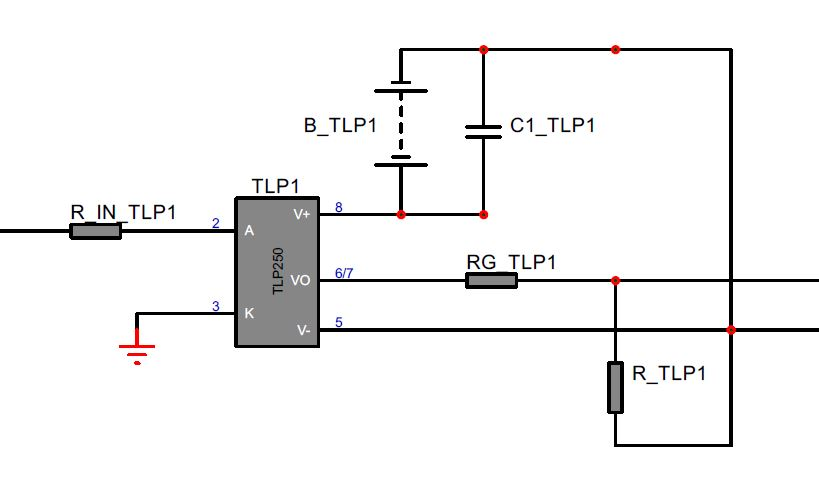
\includegraphics[width = 5in]{./Figures/Gate_driver.JPG}
		\rule{35em}{1pt}
	\caption{Circuit for TLP250}
	\label{fig:3}
\end{figure}

\begin{figure}[htbp]
	\centering
		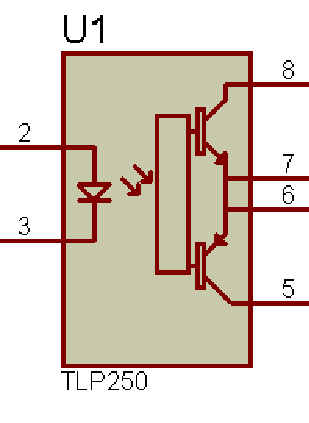
\includegraphics[width = 1.5in]{./Figures/tlp250.pdf}
		\rule{35em}{1pt}
	\caption{Inner circuit for TLP250}
	\label{fig:4}
\end{figure}
As seen from the figure\ref{fig:4} LED is connected with 2nd and 3rd pin and two BJTs are connected in series, top one to give output as $V_E$ and lower one to give discharging path.$R_in and R =1kohm $ while $R_G=10ohm$.Capacitor is of 1nF connected from pin 8 to pin 5 to stabilize the operation of the high gain linear amplifier. Failure to provide the bypassing may impair the switching property.
The pins of TLP 250 are labelled as:
\begin{itemize}
\item PIN: 2 = ANODE
\item PIN: 3 = CATHODE
\item PIN: 5 = V-/GROUND
\item PIN: 6 and 7=OUTPUT
\item PIN: 8 = V+/INPUT(15V)
\item PIN: 1 and 4 = NC
\end{itemize}
\section{H-Bridge Circuits}
There are two H-Bridge circuits used in this project[5]. By adding two H-Bridges in series so that the upper H-Bridge has DC Source = E volts and lower H-Bridge has DC Source = 3E volts, and by applying a specific switching sequence to all  switches we can obtain 9 levels in output waveform. Below the figures of all the parts are shown.

\begin{figure}[htbp]
	\centering
	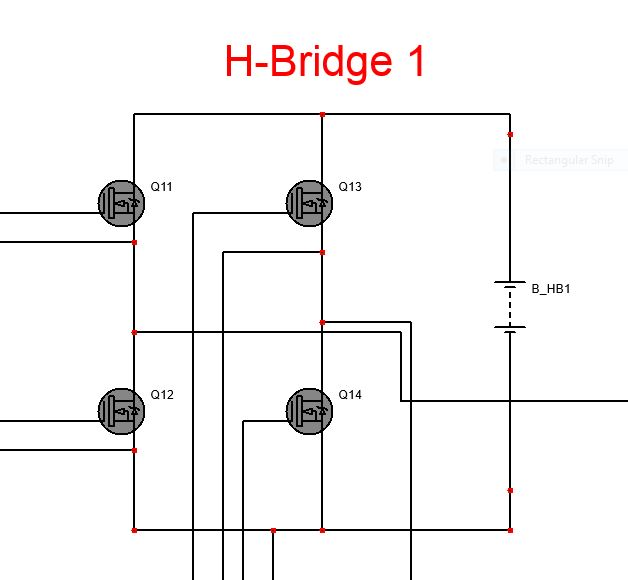
\includegraphics[width = 3.8in]{./Figures/HBridge1.JPG}
	\rule{35em}{1pt}
	\caption{H-Bridge 1 With DC Source = E volts}
	\label{fig:4}
\end{figure}
\begin{figure}[htbp]
	\centering
	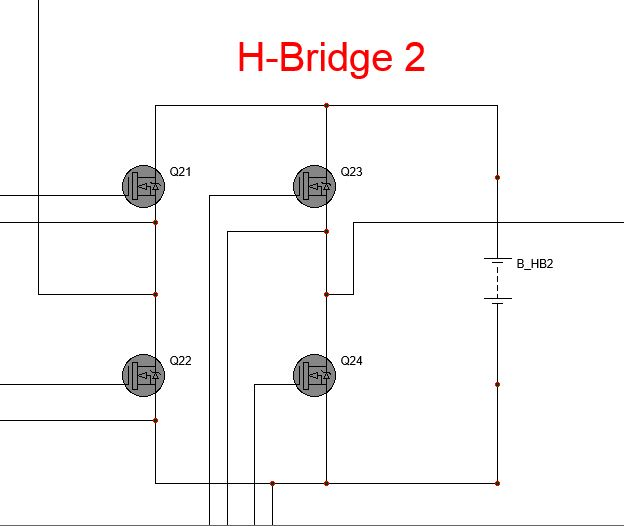
\includegraphics[width = 3.8in]{./Figures/HBridge2.JPG}
	\rule{35em}{1pt}
	\caption{H-Bridge 2 With DC Source = 3E volts}
	\label{fig:4}
\end{figure}
\begin{figure}[htbp]
	\centering
	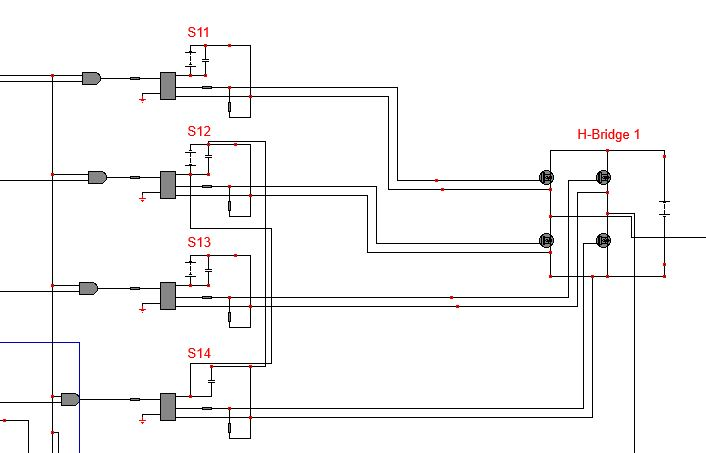
\includegraphics[width = 6in]{./Figures/C_1.JPG}
	\rule{35em}{1pt}
	\caption{H-Bridge 1 With Gate Driver Circuit}
	\label{fig:4}
\end{figure}
\begin{figure}[htbp]
	\centering
	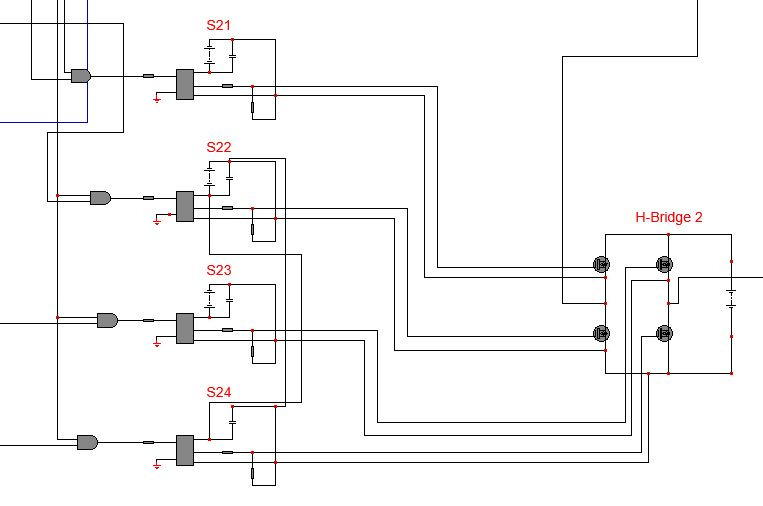
\includegraphics[width = 6in]{./Figures/C_2.JPG}
	\rule{35em}{1pt}
	\caption{H-Bridge 2 With Gate Driver Circuit}
	\label{fig:4}
\end{figure} % Experiment 1

% Chapter 1

\chapter{Simulation Results} % Write in your own chapter title
\label{Chapter5}
\lhead{Chapter 5. \emph{Simulation Results}} % Write in your own chapter title to set the page header
\section{Switching frequency}
\begin{figure}[htbp]
	\centering
	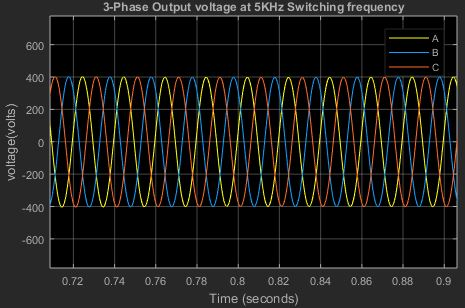
\includegraphics[width = 6in]{./Figures/5k.JPG}
	\rule{35em}{1pt}
	\caption{Output Volatge at 5KHz}
\end{figure}
\begin{figure}[htbp]
	\centering
	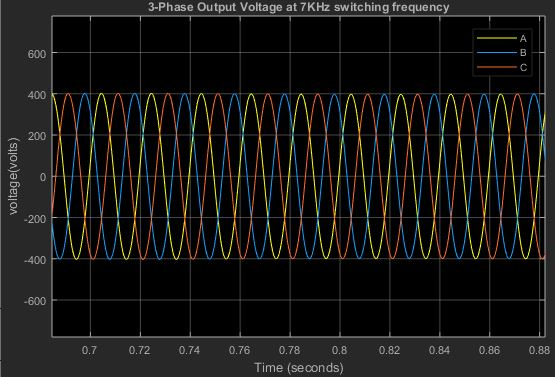
\includegraphics[width = 6in]{./Figures/7k.JPG}
	\rule{35em}{1pt}
	\caption{Output Volatge at 7KHz}
\end{figure}
\begin{figure}[htbp]
	\centering
	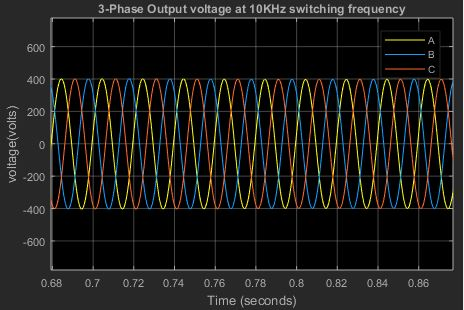
\includegraphics[width = 6in]{./Figures/10k.JPG}
	\rule{35em}{1pt}
	\caption{Output Volatge at 10KHz}
\end{figure}
\begin{figure}[htbp]
	\centering
	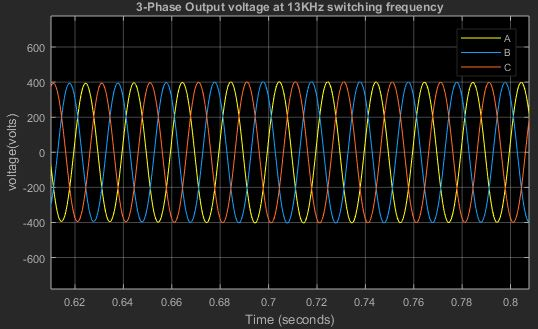
\includegraphics[width = 6in]{./Figures/13k.JPG}
	\rule{35em}{1pt}
	\caption{Output Volatge at 13KHz}
\end{figure}
\begin{figure}[htbp]
	\centering
	\includegraphics[width = 6in]{./Figures/15k.JPG}
	\rule{35em}{1pt}
	\caption{Output Volatge at 15KHz}
\end{figure}
\begin{figure}[htbp]
	\centering
	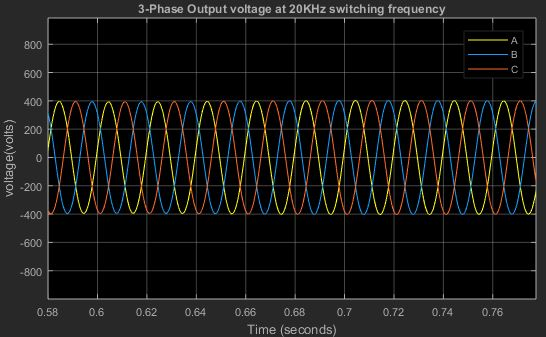
\includegraphics[width = 6in]{./Figures/20k.JPG}
	\rule{35em}{1pt}
	\caption{Output Volatge at 20KHz}
\end{figure}
\newpage
\section{Output at different rated value}
\begin{figure}[htbp]
	\centering
	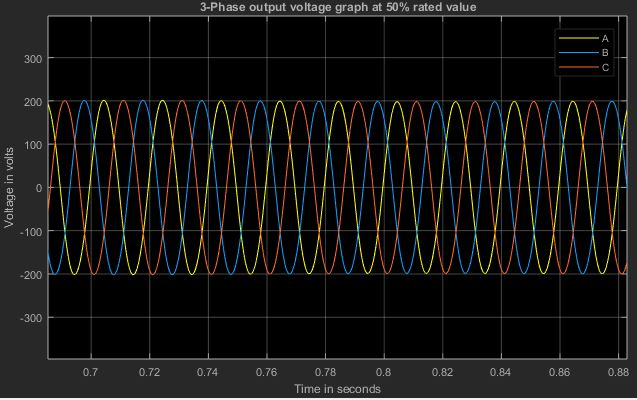
\includegraphics[width = 6in]{./Figures/50.JPG}
	\rule{35em}{1pt}
	\caption{Output Volatge at 50\% rated}
\end{figure}
\begin{figure}[htbp]
	\centering
	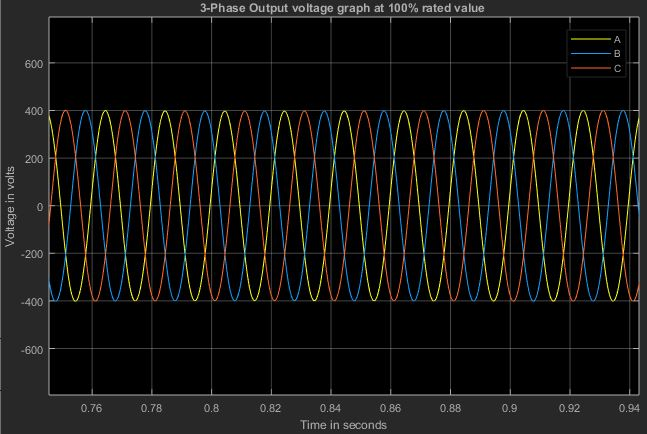
\includegraphics[width = 6in]{./Figures/100.JPG}
	\rule{35em}{1pt}
	\caption{Output Volatge at 100\% rated}
\end{figure}
\begin{figure}[htbp]
	\centering
	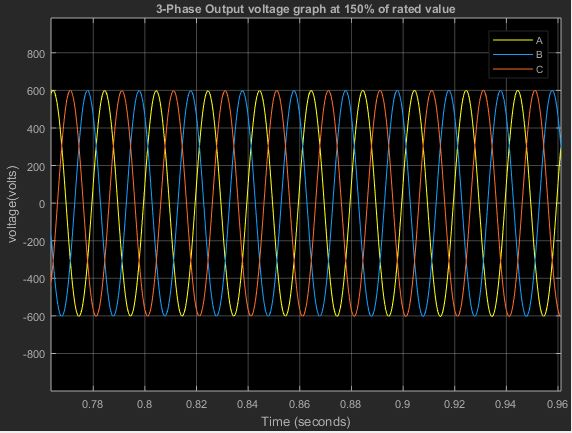
\includegraphics[width = 6in]{./Figures/150.JPG}
	\rule{35em}{1pt}
	\caption{Output Volatge at 150\% rated}
\end{figure}
\begin{figure}[htbp]
	\centering
	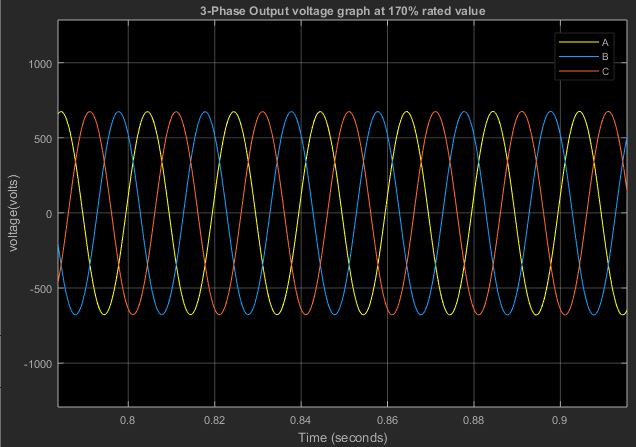
\includegraphics[width = 6in]{./Figures/170.JPG}
	\rule{35em}{1pt}
	\caption{Output Volatge at 170\% rated}
\end{figure}
\begin{figure}[htbp]
	\centering
	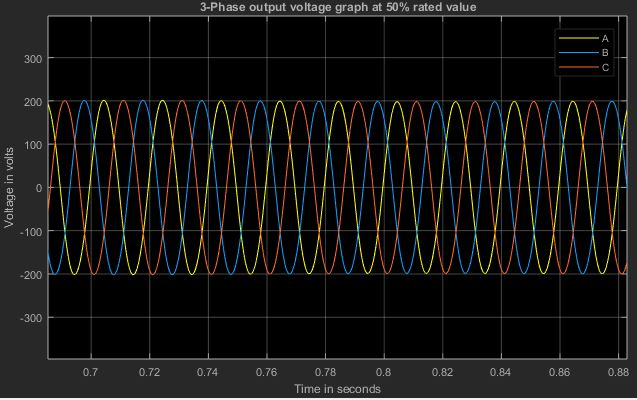
\includegraphics[width = 6in]{./Figures/50.JPG}
	\rule{35em}{1pt}
	\caption{Output Volatge at 50\% rated}
\end{figure}
\newpage
\subsection{Trend between Voltage and Index}
\begin{figure}[htbp]
	\centering
	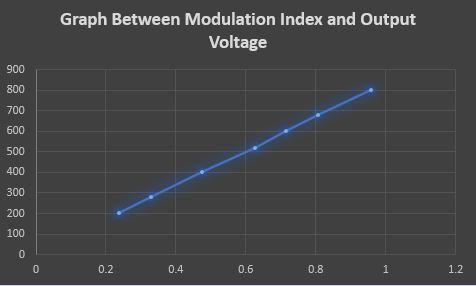
\includegraphics[width = 6in]{./Figures/mod.JPG}
	\rule{35em}{1pt}
	\caption{ModulationIndex and Output Volatge}
\end{figure}
\newpage
\section{Output Volatge at different frequencies}
\begin{figure}[htbp]
	\centering
	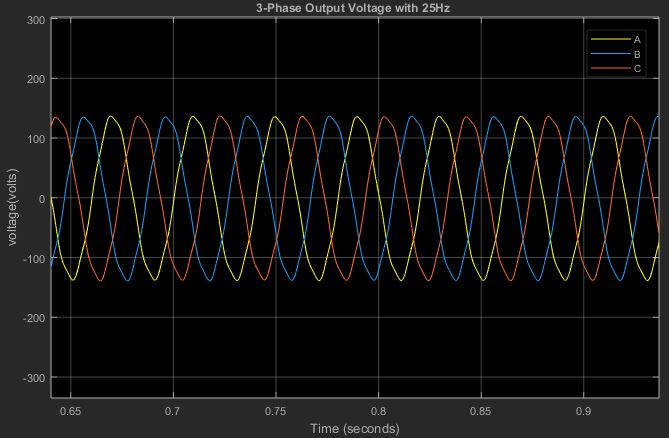
\includegraphics[width = 6in]{./Figures/25freq.JPG}
	\rule{35em}{1pt}
	\caption{Output Volatge Waveform at 25Hz}
\end{figure}
\begin{figure}[htbp]
	\centering
	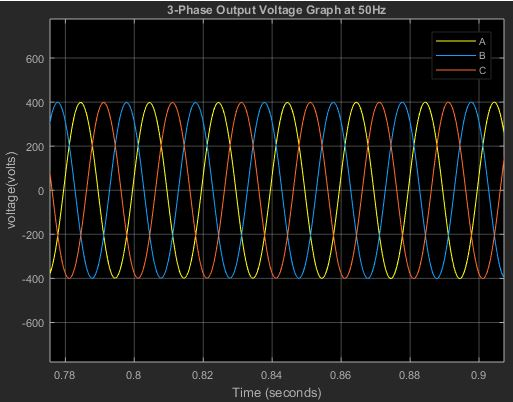
\includegraphics[width = 6in]{./Figures/50freq.JPG}
	\rule{35em}{1pt}
	\caption{Output Volatge Waveform at 50Hz}
\end{figure}
\begin{figure}[htbp]
	\centering
	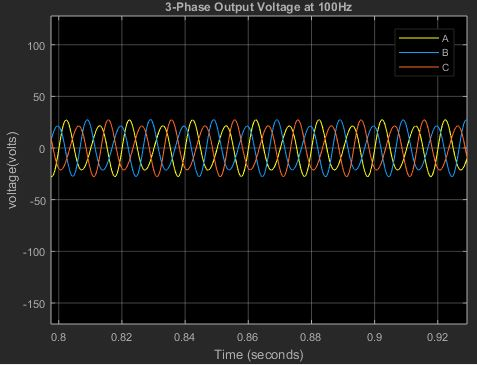
\includegraphics[width = 6in]{./Figures/100freq.JPG}
	\rule{35em}{1pt}
	\caption{Output Volatge Waveform at 100Hz}
\end{figure}
\subsection{Volatge and frequency trend}
\begin{figure}[htbp]
	\centering
	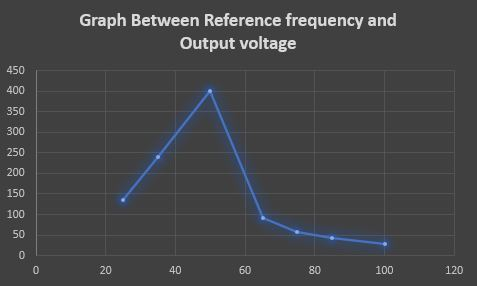
\includegraphics[width = 6in]{./Figures/graph2freq.JPG}
	\rule{35em}{1pt}
	\caption{Graph between ref. frequency and volatge}
\end{figure}
\begin{figure}[htbp]
	\centering
	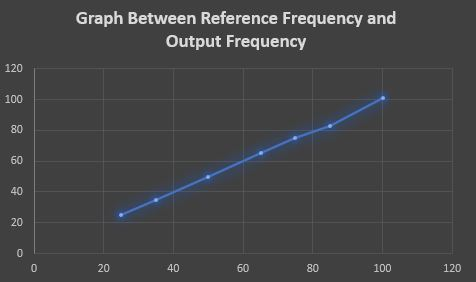
\includegraphics[width = 6in]{./Figures/graph1freq.JPG}
	\rule{35em}{1pt}
	\caption{Graph between ref. frequency and output frequency}
\end{figure}
\section{Task3}
Control the output voltage and frequency by using V/f principle. Discuss the limits of output
voltage and frequency that can be achieved. Reading is attached.
\begin{figure}[htbp]
	\centering
	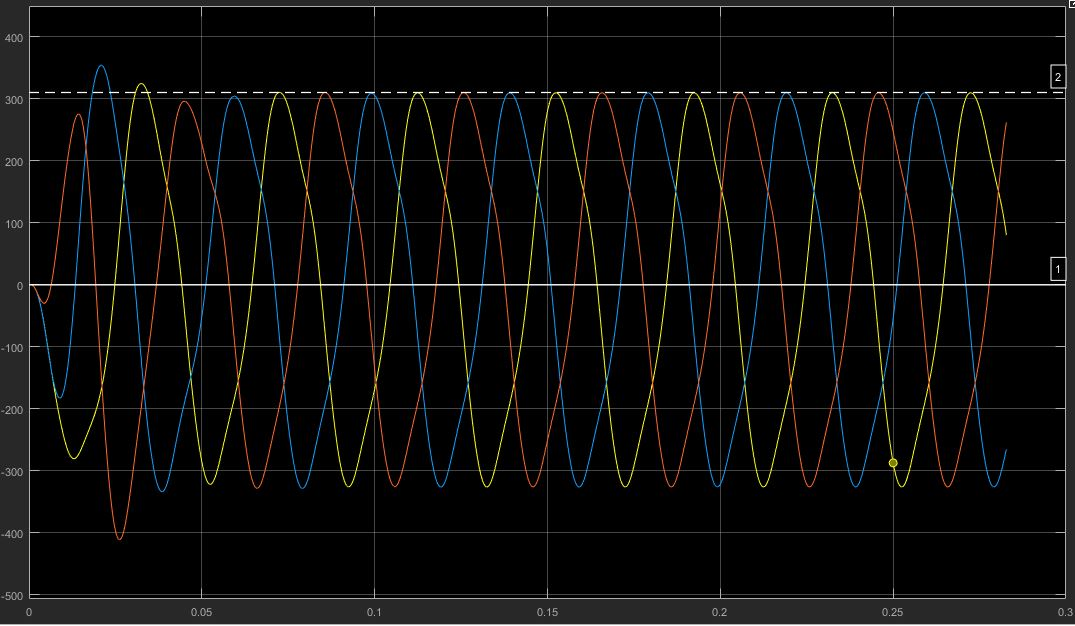
\includegraphics[width = 6in]{./Figures/Photos/task3/Task3_reading1/V313F25hz.JPG}
	\rule{35em}{1pt}
	\caption{Output volatage =313 and f = 25Hz}
\end{figure}
\begin{figure}[htbp]
	\centering
	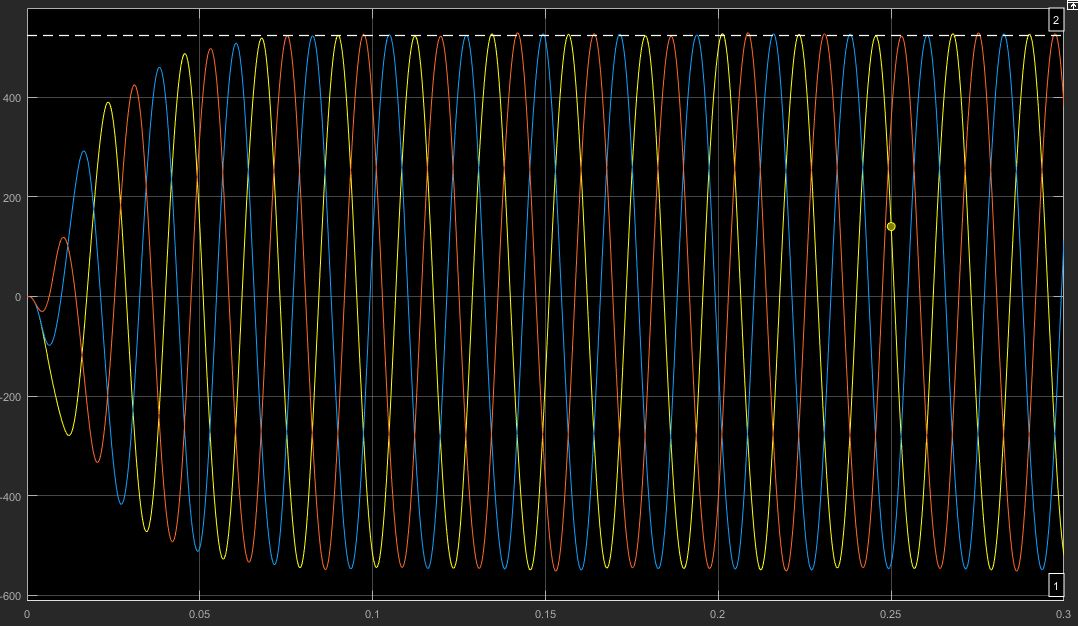
\includegraphics[width = 6in]{./Figures/Photos/task3/Task3_reading2/V525F45.JPG}
	\rule{35em}{1pt}
	\caption{Output volatage =525 and f = 45Hz}
\end{figure}
\begin{figure}[htbp]
	\centering
	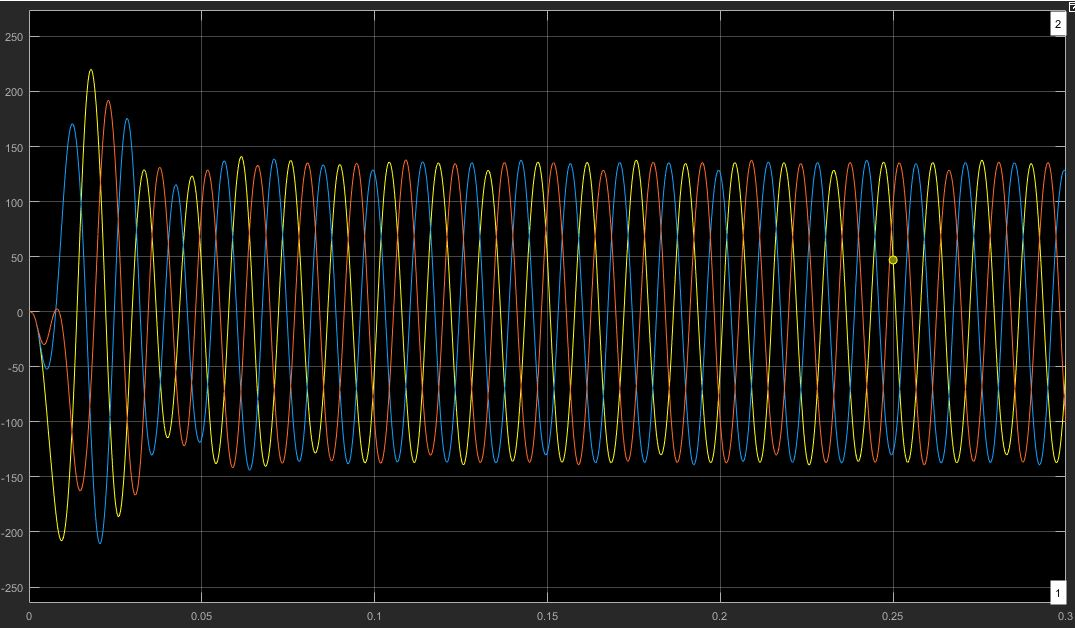
\includegraphics[width = 6in]{./Figures/Photos/task3/Task3_reading3/V132F70.JPG}
	\rule{35em}{1pt}
	\caption{Output volatage =132 and f = 70Hz}
\end{figure}
\subsection{frequency and volatge trend}
\begin{figure}[htbp]
	\centering
	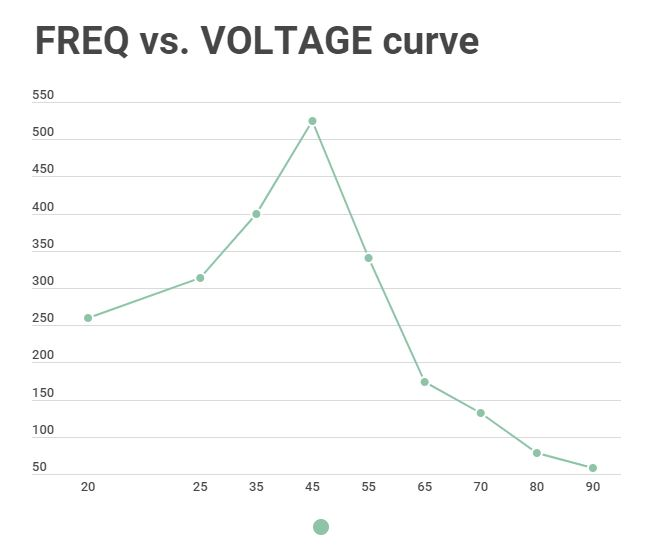
\includegraphics[width = 6in]{./Figures/Photos/task3/Graph1.JPG}
	\rule{35em}{1pt}
	\caption{trend for fixedV/f ration}
\end{figure} % Experiment 2

% Chapter 1

\chapter{Hardware Results} % Write in your own chapter title
\label{Chapter6}
\lhead{Chapter 6. \emph{Hardware Results}} % Write in your own chapter title to set the page header
\section{Output Voltage}
The output of Hardware circuit is shown below, the frequency can be verified that is 50Hz.
\begin{figure}[htbp]
	\centering
	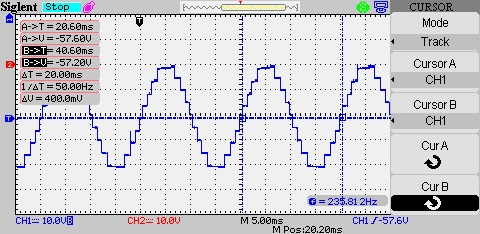
\includegraphics[width = 6in]{./Figures/Photos/Hardware/2}
	\rule{35em}{1pt}
	\caption{Output Voltage at 50Hz}
\end{figure}

The 9 levels in output waveform can be verified. The Value of voltage applied to H-Bridge 1 is 10V and the voltage applied to H-Bridge 2 is 30V i.e 3 times 10. The Switching sequence applied to all switches is shown in previous chapter. The maximum voltage is 40V and minimum voltage is -40V making it sinusoidal. The complete load parameters are shown in below figure.

\begin{figure}[htbp]
	\centering
	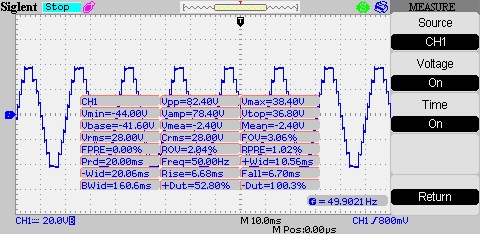
\includegraphics[width = 6in]{./Figures/Photos/Hardware/15}
	\rule{35em}{1pt}
	\caption{Output Voltage with all Load Parameters}
\end{figure}
\newpage
\section{Verification of Conduction Angles}
The conduction angles that we need to verified are given in the below table:
\begin{center}
	\begin{tabular}{ |p{4cm}||p{4cm}|  }
		\hline
		\multicolumn{2}{|c|}{Conduction Angles} \\
		\hline
		Angle & Value in Degrees\\
		\hline
		$\alpha1$ & 6$^o$\\
		\hline
		$\alpha2$ & 22$^o$\\
		\hline
		$\alpha3$ & 38$^o$\\
		\hline
		$\alpha4$ & 60$^o$\\
		\hline
	\end{tabular}
\end{center}
\subsection{Verification of $\alpha1$ }
To verify $\alpha1$ we need to calculate the time delay first step and divide it to total time period and than multiply it with 360.
From the figure shown below:

\begin{equation}
\Delta T = 0.3ms
\end{equation}
\begin{equation}
T = 20ms
\end{equation}
\begin{equation}
\alpha1 = 360*\frac{\Delta T}{T}
\end{equation}
\begin{equation}
\alpha1 = 360*\frac{0.3ms}{20ms}
\end{equation}
\begin{equation}
\alpha1 = 5.4^o
\end{equation}

\begin{figure}[htbp]
	\centering
	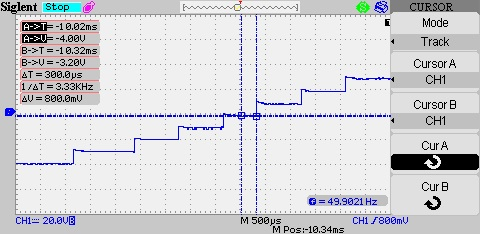
\includegraphics[width = 6in]{./Figures/Photos/Hardware/18}
	\rule{35em}{1pt}
	\caption{Verification of $\alpha1 = 6^o$}
\end{figure}
\newpage
\subsection{Verification of $\alpha2$ }
To verify $\alpha2$ we need to calculate the time delay of second step and divide it to total time period and than multiply it with 360.
From the figure shown below:

\begin{equation}
\Delta T = 1.22ms
\end{equation}

\begin{equation}
T = 20ms
\end{equation}

\begin{equation}
\alpha1 = 360*\frac{\Delta T}{T}
\end{equation}

\begin{equation}
\alpha1 = 360*\frac{1.22ms}{20ms}
\end{equation}

\begin{equation}
\alpha1 = 21.96^o
\end{equation}

\begin{figure}[htbp]
	\centering
	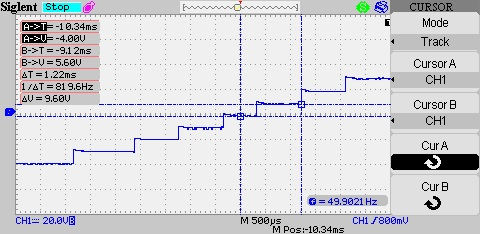
\includegraphics[width = 6in]{./Figures/Photos/Hardware/22}
	\rule{35em}{1pt}
	\caption{Verification of $\alpha2 = 22^o$}
\end{figure}

\newpage
\subsection{Verification of $\alpha3$ }
To verify $\alpha3$ we need to calculate the time delay of third step and divide it to total time period and than multiply it with 360.
From the figure shown below:

\begin{equation}
\Delta T = 2.10ms
\end{equation}

\begin{equation}
T = 20ms
\end{equation}

\begin{equation}
\alpha1 = 360*\frac{\Delta T}{T}
\end{equation}

\begin{equation}
\alpha1 = 360*\frac{2.10ms}{20ms}
\end{equation}

\begin{equation}
\alpha1 = 37.8^o
\end{equation}

\begin{figure}[htbp]
	\centering
	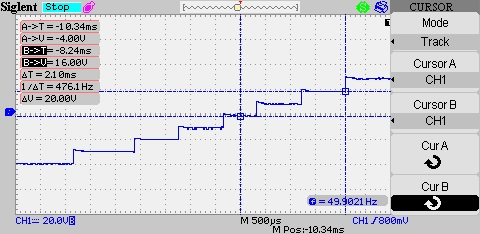
\includegraphics[width = 6in]{./Figures/Photos/Hardware/23}
	\rule{35em}{1pt}
	\caption{Verification of $\alpha3 = 38^o$}
\end{figure}

\newpage
\subsection{Verification of $\alpha4$ }
To verify $\alpha3$ we need to calculate the time delay of fourth step and divide it to total time period and than multiply it with 360.
From the figure shown below:

\begin{equation}
\Delta T = (2.10 + 1.2)ms
\end{equation}

\begin{equation}
T = 20ms
\end{equation}

\begin{equation}
\alpha1 = 360*\frac{\Delta T}{T}
\end{equation}

\begin{equation}
\alpha1 = 360*\frac{(2.10 + 1.2)ms}{20ms}
\end{equation}

\begin{equation}
\alpha1 = 59.4^o
\end{equation}

\begin{figure}[htbp]
	\centering
	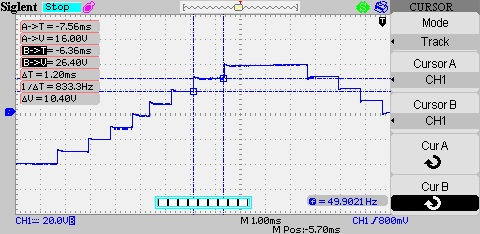
\includegraphics[width = 6in]{./Figures/Photos/Hardware/26}
	\rule{35em}{1pt}
	\caption{Verification of $\alpha4 = 60^o$}
\end{figure}
\newpage
\section{AND Operation with 10KHz PWM}
Below is the results of AND Operation with 10KHz PWM.
\begin{figure}[htbp]
	\centering
	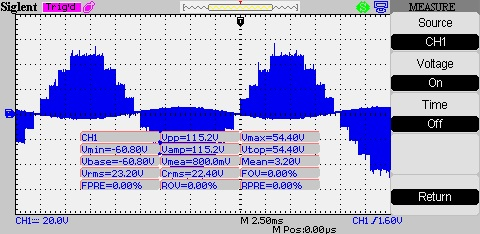
\includegraphics[width = 6in]{./Figures/Photos/Hardware/32}
	\rule{35em}{1pt}
	\caption{AND Operation with 10KHz PWM}
\end{figure}
\newpage
\section{PWM Operation}
Below is the results when PWM Operation at 10KHz is applied.
\begin{figure}[htbp]
	\centering
	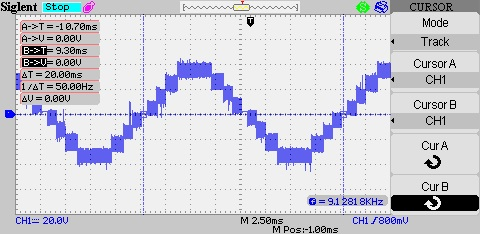
\includegraphics[width = 6in]{./Figures/Photos/Hardware/51}
	\rule{35em}{1pt}
	\caption{PWM Operation at 10KHz}
\end{figure}

\section{Frequency Control}
The frequency can be easily change by programming. Below is the result when the output frequency is 200Hz.
\begin{figure}[htbp]
	\centering
	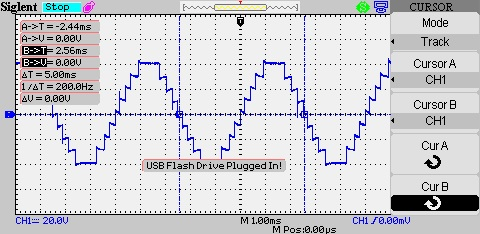
\includegraphics[width = 6in]{./Figures/Photos/Hardware/31}
	\rule{35em}{1pt}
	\caption{Frequency = 200Hz}
\end{figure}

\section{Voltage Control}
The output voltage can be controlled by taking AND Operation with a PWM signal at 10KHz frequency. Now by changing the value of duty cycle we can change the output voltage. Below are the figures showing output voltage at different duty cycles.
\newline
\newline
\textbf{Duty Cycle = 100\%}
\begin{figure}[htbp]
	\centering
	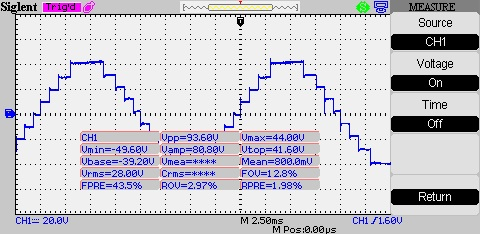
\includegraphics[width = 6in]{./Figures/Photos/Hardware/33}
	\rule{35em}{1pt}
	\caption{Duty Cycle = 100\%}
\end{figure}

\textbf{Duty Cycle = 90\%}
\begin{figure}[htbp]
	\centering
	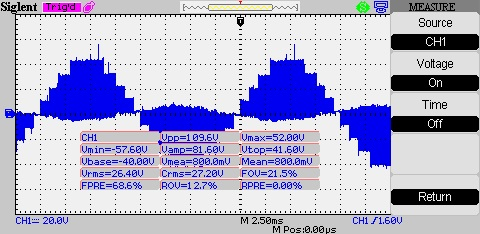
\includegraphics[width = 6in]{./Figures/Photos/Hardware/34}
	\rule{35em}{1pt}
	\caption{Duty Cycle = 90\%}
\end{figure}


\textbf{Duty Cycle = 80\%}
\begin{figure}[htbp]
	\centering
	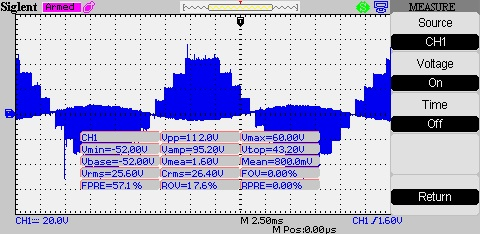
\includegraphics[width = 6in]{./Figures/Photos/Hardware/35}
	\rule{35em}{1pt}
	\caption{Duty Cycle = 80\%}
\end{figure}


\textbf{Duty Cycle = 70\%}
\begin{figure}[htbp]
	\centering
	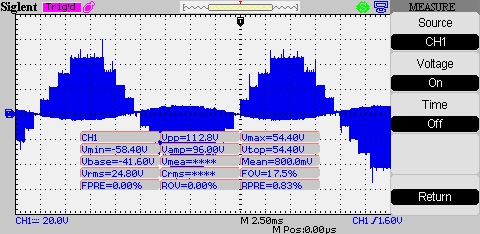
\includegraphics[width = 6in]{./Figures/Photos/Hardware/36}
	\rule{35em}{1pt}
	\caption{Duty Cycle = 70\%}
\end{figure}


\textbf{Duty Cycle = 60\%}
\begin{figure}[htbp]
	\centering
	\includegraphics[width = 6in]{./Figures/Photos/Hardware/37}
	\rule{35em}{1pt}
	\caption{Duty Cycle = 60\%}
\end{figure}

\newpage
\textbf{Duty Cycle = 50\%}
\begin{figure}[htbp]
	\centering
	\includegraphics[width = 6in]{./Figures/Photos/Hardware/38}
	\rule{35em}{1pt}
	\caption{Duty Cycle = 50\%}
\end{figure}

\newpage
\textbf{Duty Cycle = 40\%}
\begin{figure}[htbp]
	\centering
	\includegraphics[width = 6in]{./Figures/Photos/Hardware/39}
	\rule{35em}{1pt}
	\caption{Duty Cycle = 40\%}
\end{figure}


\textbf{Duty Cycle = 30\%}
\begin{figure}[htbp]
	\centering
	\includegraphics[width = 6in]{./Figures/Photos/Hardware/40}
	\rule{35em}{1pt}
	\caption{Duty Cycle = 30\%}
\end{figure}

\newpage
\textbf{Duty Cycle = 20\%}
\begin{figure}[htbp]
	\centering
	\includegraphics[width = 6in]{./Figures/Photos/Hardware/41}
	\rule{35em}{1pt}
	\caption{Duty Cycle = 20\%}
\end{figure}


\textbf{Duty Cycle = 10\%}
\begin{figure}[htbp]
	\centering
	\includegraphics[width = 6in]{./Figures/Photos/Hardware/42}
	\rule{35em}{1pt}
	\caption{Duty Cycle = 10\%}
\end{figure}

\newpage
\textbf{Duty Cycle = 5\%}
\begin{figure}[htbp]
	\centering
	\includegraphics[width = 6in]{./Figures/Photos/Hardware/43}
	\rule{35em}{1pt}
	\caption{Duty Cycle = 5\%}
\end{figure}

\textbf{Duty Cycle = 2\%}
\begin{figure}[htbp]
	\centering
	\includegraphics[width = 6in]{./Figures/Photos/Hardware/44}
	\rule{35em}{1pt}
	\caption{Duty Cycle = 2\%}
\end{figure}
\newpage
\textbf{Duty Cycle = 1\%}
\begin{figure}[htbp]
	\centering
	\includegraphics[width = 6in]{./Figures/Photos/Hardware/45}
	\rule{35em}{1pt}
	\caption{Duty Cycle = 1\%}
\end{figure}

\textbf{Duty Cycle = 0\%}
\begin{figure}[htbp]
	\centering
	\includegraphics[width = 6in]{./Figures/Photos/Hardware/46}
	\rule{35em}{1pt}
	\caption{Duty Cycle = 0\%}
\end{figure}
\subsection{Table }
\begin{center}
	\begin{tabular}{ |p{4cm}||p{4cm}|  }
		\hline
		\multicolumn{2}{|c|}{Vriaion of $V_output$(RMS) w.r.t Duty cycle} \\
		\hline
		Duty Cycle (\%) & $V_{output}$(RMS)\\
		\hline
		100 & 28 \\
		\hline
        90 & 26.4\\
        \hline
        80 & 25.6 \\
        \hline
        70 & 24.8 \\
        \hline
        60 & 23.20 \\
        \hline
        50 & 21.6 \\
        \hline
        40 & 20.8 \\
        \hline
        30 & 17.6 \\
        \hline	
        20 & 14.4 \\
        \hline	
        10 & 10.4 \\
        \hline
        5 & 8 \\
        \hline
        2 & 4.8 \\
        \hline
        1 & 3.2 \\
        \hline
        0 & 0.8 \\
        \hline
	\end{tabular}
\end{center}

\subsection{Relation Between Duty Cycle and V$_{rms}$}
\begin{figure}[htbp]
	\centering
	\includegraphics[width = 5in]{./Figures/p_d_v}
	\rule{35em}{1pt}
	\caption{Relation Between Duty Cycle and V$_{rms}$}
\end{figure}

\section{Voltage and Current Parameters}
Below is the load parameters when 100W load is connected at the output terminals.
\begin{equation}
V_{H-Bridge-1} = 50V
\end{equation} 
\begin{equation}
V_{H-Bridge-2} = 150V
\end{equation} 
\begin{equation}
Vout_{rms} = 150V
\end{equation} 
\begin{equation}
Iout_{rms} = 2.205A
\end{equation} 
\begin{center}
	\begin{tabular}{ |p{4cm}||p{4cm}|p{4cm}|  }
		\hline
		\multicolumn{3}{|c|}{Load Parameters} \\
		\hline
		Component & Voltage & Current \\
		\hline
		Isolated Supplies for Gate Driver & 15V & 14mA\\
				\hline
		TLP250 Input (Gate Driver) & 3.3V & 15mA\\
				\hline
		TLP250 Output (Gate Driver) & 15V & 14mA\\
				\hline
		IRF450 (H-Bridge-1) & 50V$_{rms}$ & 0.7352A\\
				\hline
		IRF450 (H-Bridge-2) & 150V$_{rms}$ & 2.205A\\
				\hline
		STM32F4 (GPIO Pins) & 3.3V & 15mA\\
		\hline
	\end{tabular}
\end{center}
 % Results and Discussion

% Chapter 1

\chapter{Conclusion} % Write in your own chapter title
\label{Chapter5}
\lhead{Chapter 5. \emph{Conclusion}} % Write in your own chapter title to set the page header
In this paper, a three-phase 9-level cascaded multilevel
inverter with output voltage and frequency control has been
presented, achieving output signals with high quality and very
low THD. The phase shift and disposition orders of modulating signals are
another important point of design to reduce THD of line
current and voltages.The DC level of H-bridges has been intended to construct
output levels and dual DC supplies at Vdc:3Vdc ratio have
been constituted 9-level output voltage. The proposed model
has been tested and compared to its precedent conventional
models for THD rates and switching bandwidth. The
measurement results have presented perfect outcomes on
THD analysis. It is also seen that the switching frequency is directly effective
on THD. % Conclusion

%% ----------------------------------------------------------------
% Now begin the Appendices, including them as separate files

\addtocontents{toc}{\vspace{2em}} % Add a gap in the Contents, for aesthetics

\appendix % Cue to tell LaTeX that the following 'chapters' are Appendices

% Appendix A

\chapter{Code for Project}
\label{AppendixA}
\lhead{Appendix A. \emph{Code for Project}}
\section{STM32F4 Code}
\begin{lstlisting}
/* Includes */
#include "stm32f4xx.h"
#include "stm32f401_discovery.h"
#include "math.h"
/*
PD0 -> S11
PD1 -> S13
PD2 -> S21
PD3 -> S23
PD4 -> S12
PD5 -> S14
PD6 -> S22
PD7 -> S24
*/

const int sine_table[50] = { 2089, 1052, 0, 1052, 2088, 3092, 4046, 4937, 5750,
	6472, 7092, 7600, 7988, 8251, 8383, 8383, 8251, 7988, 7600, 7092, 6472,
	5750, 4937, 4046, 3092, 2089, 1052, 0, 1052, 2088, 3092, 4046, 4937,
	5750, 6472, 7092, 7600, 7988, 8251, 8383, 8383, 8251, 7988, 7600, 7092,
	6472, 5750, 4937, 4046, 3092 };

const int hex_values[17] = { 0xF0, 0xF0, 0xE1, 0x96, 0x87, 0xA5, 0x87, 0x96,
	0xE1, 0xF0, 0xD2, 0x69, 0x4B, 0x5A, 0x4B, 0x69, 0xD2 };
uint16_t arr_values[17] = { 0 };
uint8_t s11, s13, s21, s23, ss;
uint8_t index0 = 1, sin_index = 0;
uint16_t duty = 100;
float m_a = 1.0f;

void timer3_Init() {
	RCC_APB1PeriphClockCmd(RCC_APB1Periph_TIM3, ENABLE);
	TIM_TimeBaseInitTypeDef tim;
	tim.TIM_Period = arr_values[0] - 1;
	tim.TIM_Prescaler = 9;
	tim.TIM_ClockDivision = TIM_CKD_DIV1;
	tim.TIM_CounterMode = TIM_CounterMode_Up;
	TIM_TimeBaseInit(TIM3, &tim);
	
	NVIC_InitTypeDef nvic;
	nvic.NVIC_IRQChannel = TIM3_IRQn;
	nvic.NVIC_IRQChannelCmd = ENABLE;
	NVIC_Init(&nvic);
	
	TIM_ITConfig(TIM3, TIM_IT_Update, ENABLE);
	
	TIM_ARRPreloadConfig(TIM3, ENABLE);
	
	TIM_Cmd(TIM3, ENABLE);
}

void timer2_Init() {
	RCC_APB1PeriphClockCmd(RCC_APB1Periph_TIM2, ENABLE);
	TIM_TimeBaseInitTypeDef tim;
	tim.TIM_Period = 33599;
	tim.TIM_Prescaler = 0;
	tim.TIM_ClockDivision = TIM_CKD_DIV1;
	tim.TIM_CounterMode = TIM_CounterMode_Up;
	TIM_TimeBaseInit(TIM2, &tim);
	
	NVIC_InitTypeDef nvic;
	nvic.NVIC_IRQChannel = TIM2_IRQn;
	nvic.NVIC_IRQChannelCmd = ENABLE;
	NVIC_Init(&nvic);
	TIM_ITConfig(TIM2, TIM_IT_Update, ENABLE);
	
	TIM_ARRPreloadConfig(TIM2, ENABLE);
	TIM_Cmd(TIM2, ENABLE);
}

void init_GPIOs() {
	RCC_AHB1PeriphClockCmd(RCC_AHB1Periph_GPIOD, ENABLE);
	RCC_AHB1PeriphClockCmd(RCC_AHB1Periph_GPIOA, ENABLE);
	
	GPIO_InitTypeDef gpio;
	
	gpio.GPIO_Pin = GPIO_Pin_0 | GPIO_Pin_1 | GPIO_Pin_2 | GPIO_Pin_3
	| GPIO_Pin_4 | GPIO_Pin_5 | GPIO_Pin_6 | GPIO_Pin_7;
	gpio.GPIO_Mode = GPIO_Mode_OUT;
	GPIO_Init(GPIOD, &gpio);
	
	gpio.GPIO_Pin = GPIO_Pin_0;
	gpio.GPIO_Mode = GPIO_Mode_IN;
	GPIO_Init(GPIOA, &gpio);
}

void PWM_Init() {
	
	RCC_APB1PeriphClockCmd(RCC_APB1Periph_TIM4, ENABLE);
	RCC_AHB1PeriphClockCmd(RCC_AHB1Periph_GPIOD, ENABLE);
	
	GPIO_InitTypeDef gpio;
	gpio.GPIO_Pin = GPIO_Pin_12;
	gpio.GPIO_Mode = GPIO_Mode_AF;
	gpio.GPIO_Speed = GPIO_Speed_100MHz;
	GPIO_Init(GPIOD, &gpio);
	
	GPIO_PinAFConfig(GPIOD, GPIO_PinSource12, GPIO_AF_TIM4);
	
	TIM_TimeBaseInitTypeDef tim;
	tim.TIM_Period = 8399;
	tim.TIM_Prescaler = 0;
	tim.TIM_ClockDivision = TIM_CKD_DIV1;
	tim.TIM_CounterMode = TIM_CounterMode_Up;
	TIM_TimeBaseInit(TIM4, &tim);
	
	TIM_OCInitTypeDef tim_oc;
	tim_oc.TIM_OCMode = TIM_OCMode_PWM1;
	tim_oc.TIM_OCPolarity = TIM_OCPolarity_High;
	tim_oc.TIM_OutputState = TIM_OutputState_Enable;
	tim_oc.TIM_Pulse = 4199;
	TIM_OC1Init(TIM4, &tim_oc);
	TIM_OC1PreloadConfig(TIM4, TIM_OCPreload_Enable);
	TIM_Cmd(TIM4, ENABLE);
	
}

void init_ARR() {
	double p = 20; // 20ms, 50Hz
	double ca[4] = { 6, 22, 38, 60 }; //{ 6, 22, 38, 60 }; // {9.8409, 20.3828, 38.4054, 60.4164}
	double delay_time[17] = { 0 };
	double sum = 0;
	int i = 0;
	for (i = 0; i < 17; i++) {
		if (i < 4) {
			delay_time[i] = (ca[i] / 360) * p - sum;
			sum += delay_time[i];
		} else if (i == 4) {
			delay_time[i] = (p / 2 - (ca[3] / 360) * p) - sum;
		} else if (i > 4 && i < 8) {
			delay_time[i] = delay_time[8 - i];
		} else if (i == 8) {
			delay_time[i] = delay_time[0] * 2;
		} else if (i > 8 && i < 16) {
			delay_time[i] = delay_time[i - 8];
		} else if (i == 16) {
			delay_time[16] = delay_time[0];
		}
	}
	for (i = 0; i < 17; i++) {
		arr_values[i] = lround((double) (delay_time[i] * 8400));
	}
}

int main(void) {
	ss = 1;
	int index1 = 0;
	uint16_t CCR_value = 0;
	uint8_t AND = 2;
	uint8_t spwm = 0;
	init_GPIOs();
	init_ARR();
	PWM_Init();
	timer3_Init();
	if (spwm) {
		timer2_Init();
	}
	while (1) {
		if (!spwm) {
			CCR_value = (uint16_t) (((float) (duty / 100.0)) * 8400);
			TIM4->CCR1 = CCR_value;
		}
		index1 = index0 - 1;
		if (index1 < 0) {
			index1 = 16;
		}
		ss = GPIO_ReadInputDataBit(GPIOA, GPIO_Pin_0);
		
		if (AND == 2) {
			GPIO_Write(GPIOD, (hex_values[index1]));
		}
		if (AND == 1) {
			GPIO_Write(GPIOD, (hex_values[index1] * ss));
		} else if (AND == 0) {
			
			GPIO_Write(GPIOD, (hex_values[index1]));
			
			if (index1 == 6 || index1 == 7 || index1 == 14 || index1 == 15) {
				if (ss == 0) {
					GPIO_Write(GPIOD, (hex_values[index1 + 1]));
				}
			}
			if (index1 == 2 || index1 == 8 || index1 == 10 || index1 == 16) {
				GPIO_Write(GPIOD, (hex_values[index1] * ss));
			}
			if (index1 == 3 || index1 == 4 || index1 == 5 || index1 == 11
			|| index1 == 12 || index1 == 13) {
				if (ss == 0) {
					GPIO_Write(GPIOD, (hex_values[index1 - 1]));
				}
			}
		}
		/*	s11 = GPIO_ReadOutputDataBit(GPIOD, GPIO_Pin_0);
		s13 = GPIO_ReadOutputDataBit(GPIOD, GPIO_Pin_1);
		s21 = GPIO_ReadOutputDataBit(GPIOD, GPIO_Pin_2);
		s23 = GPIO_ReadOutputDataBit(GPIOD, GPIO_Pin_3);*/
	}
}

void TIM3_IRQHandler() {
	if (TIM_GetITStatus(TIM3, TIM_IT_Update)) {
		TIM_ClearITPendingBit(TIM3, TIM_IT_Update);
		
		TIM3->ARR = arr_values[index0] - 1;
		index0 = (index0 + 1) % 17;
		
	}
}

void TIM2_IRQHandler() {
	if (TIM_GetITStatus(TIM2, TIM_IT_Update)) {
		TIM_ClearITPendingBit(TIM2, TIM_IT_Update);
		TIM4->CCR1 = (uint16_t) (m_a * sine_table[sin_index]);
		sin_index = (sin_index + 1) % 50;
	}
}

/*
* Callback used by stm32f401_discovery_audio_codec.c.
* Refer to stm32f401_discovery_audio_codec.h for more info.
*/
void EVAL_AUDIO_TransferComplete_CallBack(uint32_t pBuffer, uint32_t Size) {
	/* TODO, implement your code here */
	return;
}

/*
* Callback used by stm32f401_discovery_audio_codec.c.
* Refer to stm32f401_discovery_audio_codec.h for more info.
*/
uint16_t EVAL_AUDIO_GetSampleCallBack(void) {
	/* TODO, implement your code here */
	return -1;
}
\end{lstlisting}

\section{MATLAB CODE}
\subsection{Switching Sequence Generator:}
\begin{lstlisting}
clear;clc;
%% Sequence Generator
% This script generates 4 switching sequences o11, 013, o21, o23 for
% switches Q11, Q13, Q21, Q23 respectively. o12, o14, o22 and o24 can be
% obtain by inverting o11, 013, o21, o23 respectively
% -------------------
%% Input
options.Interpreter = 'tex';
% Include the desired Default answer
options.Default = 'No PWM';
% Use the TeX interpreter in the question
qstring = 'Please Select Operation Mode?';
choice = questdlg(qstring,'Operation Mode',...
'No PWM','PWM Operation','SPWM Operation',options);

% Defining Variables
d = 100; % Duty
ma = 1.0; % Modulation Index

% Handle response
switch choice
case 'No PWM'
option = 0;
case 'PWM Operation'
option = 1;
answer = inputdlg("Enter Duty Value: ");
d = str2double(answer{1}); % Store Duty Value
case 'SPWM Operation'
option = 2;
answer = inputdlg("Enter Value of Modulaion Index: ");
ma = str2double(answer{1}); % Store Vlaue of Modulation Index
end
%% Initialization

Fs = 10000; % Samples per Period
p = 20e-3; % Time Period. (Variable Frequency can be obtain by changing period value)
t = linspace(0, p, Fs); % Time axis
duty = d; % From User Input
sw_freq = 10e3; % Switching Frequency for PWM Operation
if (option == 2) % Sine PWM
pwm = SPWM(sw_freq, t, ma);
end
if (option == 1) % PWM
pwm = (1 + square(2*pi*sw_freq*t, duty))/2;
end
if (option == 0) % No PWM
pwm = ones(1, Fs);
end
o11 = zeros(1, Fs);
o13 = zeros(1, Fs);
o21 = zeros(1, Fs);
o23 = zeros(1, Fs);
%% Data

% Conduction Angles or Switching Angles in Degrees
cond_angles = [6 22 38 60]; %(for SHE PWM)[9.8409 20.3828 38.4054 60.4164]; 

% Switching Sequence with minimum transitions
s11 = [0 1 0 1 1 1 0 1 0 0 1 1 0 1 1 0 0];
s13 = [0 0 1 1 0 1 1 0 0 1 0 1 1 1 0 1 0];
s21 = [0 0 1 1 1 1 1 0 0 0 0 0 0 0 0 0 0];
s23 = [0 0 0 0 0 0 0 0 0 0 1 1 1 1 1 0 0];

%% Calculations
%  Calculating Time Axis values of all steps based on conduction angles
time_value = [
(cond_angles(1)/360)*p
((cond_angles(2)/360)*p)
((cond_angles(3)/360)*p)
((cond_angles(4)/360)*p)
((p/2 - (cond_angles(4)/360)*p))
((p/2 - (cond_angles(3)/360)*p))
((p/2 - (cond_angles(2)/360)*p))
((p/2 - (cond_angles(1)/360)*p))
((p/2 + (cond_angles(1)/360)*p))
((p/2 + (cond_angles(2)/360)*p))
((p/2 + (cond_angles(3)/360)*p))
((p/2 + (cond_angles(4)/360)*p))
((p - (cond_angles(4)/360)*p))
((p - (cond_angles(3)/360)*p))
((p - (cond_angles(2)/360)*p))
((p - (cond_angles(1)/360)*p))
p
];
%% Output Generation
% Based on conduction angles generating sequences for Q11, Q13, Q21 and
% Q23
j = 1;
for i = 1:Fs
o11(i) = s11(j)*pwm(i);
o13(i) = s13(j)*pwm(i);
o21(i) = s21(j)*pwm(i);
o23(i) = s23(j)*pwm(i);

if t(i) > time_value(j)
j = j + 1;
end
end
\end{lstlisting}

\subsection{Sine PWM Generator}
\begin{lstlisting}
function y = SPWM(f, t, ma)
counter = 1;
y = zeros(1, length(t));
table = zeros(1, 200);
for angle = 0:0.9:179
table(counter) = ma*100*sind(angle);
counter = counter + 1;
end
sin_table = [table table];
del = length(t)/length(sin_table);
lower = 1;
upper = del;
angle = 1;
for counter = 1:del:length(t)
y(lower:upper) = (1 + square(2*pi*f*t(lower:upper), sin_table(angle)))/2;
lower = upper + 1;
upper = upper + del;
angle = angle + 1;
end

\end{lstlisting}

\subsection{SHE PWM}
\begin{lstlisting}
clear; clc;
% x = [9.8409   20.3828   38.4054   60.4164]
x0 = [6 22 38 60];
fun = @set_of_equations;
options = optimoptions('fsolve', 'MaxFunctionEvaluations', 20000, 'OptimalityTolerance', 1e-6, 'StepTolerance', 1e-6, 'MaxIterations', 2000, 'PlotFcn', @optimplotfval);
x = fsolve(fun, x0, options);
\end{lstlisting}
\subsection{Equations}
\begin{lstlisting}
function F = set_of_equations(x)
F = zeros(1,4);
F(1) = cosd(x(1)) + cosd(x(2)) + cosd(x(3)) + cosd(x(4)) - 3.2;
F(2) = cosd(5*x(1)) + cosd(5*x(2)) + cosd(5*x(3)) + cosd(5*x(4));
F(3) = cosd(7*x(1)) + cosd(7*x(2)) + cosd(7*x(3)) + cosd(7*x(4));
F(4) = cosd(11*x(1)) + cosd(11*x(2)) + cosd(11*x(3)) + cosd(11*x(4));
\end{lstlisting}	% Appendix Title

%\input{./Chapters/AppendixB} % Appendix Title

%\input{./Chapters/AppendixC} % Appendix Title

\addtocontents{toc}{\vspace{2em}}  % Add a gap in the Contents, for aesthetics
\backmatter

%% ----------------------------------------------------------------
%\label{References}
%\lhead{\emph{References}}  % Change the left side page header to "References"

%\bibliographystyle{plainnat}  % Use "unsrtnat" BibTeX style for formatting the references

%\bibliography{references}  % The references information are stored in the file named "references.bib"

\end{document}  % The End
%% ----------------------------------------------------------------
